\documentclass[aspectratio=169,t]{beamer}
\usepackage[utf8]{inputenc}
\usepackage[T1]{fontenc}
\usepackage[english]{babel}
\usepackage{hyperref}
\usepackage{tikz}

\usepackage{graphicx}
\usepackage{epstopdf}
\usepackage{multirow}

\usepackage{psfrag}
\usepackage{pgfplots}
\usepackage{framed}
\usepackage{xcolor}
\usepackage{booktabs}
\usepackage{caption}
\usepackage{epstopdf}
\usepackage{amsmath}
\usepackage{tabularx}
\usepackage[]{bookmark}
%\usepackage[3D]{movie15}
%\usepackage{media9}
\usepackage[binary-units,abbreviations]{siunitx}
\usepackage[textfont=normalsize, labelfont=normalsize, justification=centering]{subcaption}
\usepackage{marvosym}
\usepackage{calc}
\usepackage{color, colortbl}
\usepackage[]{svg} 
\usepackage[]{trfsigns} 
\usepackage[nomessages]{fp}
\usepackage[]{csquotes}\MakeOuterQuote{"}
\usepackage{tabto}
\selectcolormodel{rgb}

\makeatletter
\def\beamer@calltheme#1#2#3{\def\beamer@themelist{#2}
	\@for\beamer@themename:=\beamer@themelist\do
	{\usepackage[{#1}]{\beamer@themelocation/#3\beamer@themename}}}
\def\usefolder#1{\def\beamer@themelocation{#1}}
\def\beamer@themelocation{}
\usefolder{theme}

\usetikzlibrary{matrix,
	decorations.pathreplacing,
	calc,
	positioning,
	external,
	3d,
	shapes,
	arrows,
	pgfplots.statistics}
\pgfplotsset{compat=1.16}
\tikzstyle{faunode}=[rounded corners, draw=faublue, fill=faublue!10,  align=center, inner sep=0.3cm, line width=0.4mm]
\tikzstyle{fauellipseFixedWidth}=[ellipse, draw=faublue, fill=faublue!10,  align=center, inner sep=0.3cm, line width=0.4mm, minimum width=3cm]
\tikzstyle{fauellipse}=[ellipse, draw=faublue, fill=faublue!10,  align=center, inner sep=0.3cm, line width=0.4mm]
\tikzstyle{fauarrow}=[draw=faublue,->, line width=0.4mm]
\tikzstyle{fauline}=[draw=faublue, line width=0.4mm]


\usepackage[backend=bibtex,sorting=none,doi=true,style=phys]{biblatex}
%\usepackage[]{biblatex}
\bibliography{./references}

% Themes:
%  - fau:          FAU theme
%  - fau-tf:       TechFak FAU theme
%  - fau-tf-lme:   TechFak LME FAU theme
%  - fau-tf-aibe:  TechFak AIBE FAU theme
%
% Options:
%  - image:        Cover image on title page
%  - plain:        Plain title page
%  - longtitle:    Title page layout for long title
% \usetheme[longtitle]{fau-tf-lme}
\usetheme[longtitle]{fau-tf-aibe}

% END of THEME SETTINGS
% --------------------------------------------------------------------------------------------------------------------------------------------------------------------------

\sisetup{
exponent-product =\ensuremath{{\,\cdot\,}}
}

% Enable semi-transparent animation preview
\setbeamercovered{transparent}
\setbeamertemplate{blocks}[rounded]
\captionsetup{labelformat=empty,labelsep=none, labelfont=normalsize, justification=centering}


\newcommand\Wider[2][1.0cm]{%
\makebox[\linewidth][c]{%
  \begin{minipage}{\dimexpr\textwidth+#1\relax}
  \raggedright#2
  \end{minipage}%
  }%
}


\let\origitem\item
\renewcommand{\item}{\normalfont\origitem}
\newcommand{\bluefat}[1]{\textcolor{faublue}{\textbf{#1}}}
\newcommand{\bolditem}{\normalfont\origitem\bfseries}
\newcommand{\question}{{\bf Question: }}
\newcommand{\answer}{{\bf Answer: }}
\newcommand{\myExample}{{\bf Example }}
\newcommand{\real}{\mbox{${\mathbb R}$}}
\definecolor{defColor}{rgb}{0.8,0.87,0.97}
\definecolor{defColorT}{rgb}{0,0,0}
\definecolor{defColorF}{rgb}{1,1,1}
\newenvironment{myDefinition}{%
	\def\FrameCommand{\fboxsep=\FrameSep{} \fcolorbox{defColorF}{defColor}}%
	\color{defColorT}\MakeFramed{\FrameRestore{}}}%
{\endMakeFramed}

% Title page
\title[Medical Engineering II]{Medical Engineering - Imaging Systems}

\author{Prof.\ Dr. Bernhard Kainz \and Prof.\ Dr. Florian Knoll}
\date{SS 2024}
\institute{IDEA Lab and Computational Imaging Lab at Dept. AIBE}

\newcommand{\password}{\texttt{mt2\_ss22}}


\AtBeginSection[]{
	{
		\setbeamertemplate{footline}{}
		\begin{frame}[noframenumbering]{\insertsubtitle}
			 \tableofcontents[currentsection]
		\end{frame} 
	}
}
\AtBeginSubsection[]{
	{

		\setbeamertemplate{footline}{}
		\begin{frame}[noframenumbering]{\insertsubtitle}
			 \tableofcontents[currentsection, currentsubsection]
		\end{frame} 
	}
}


\selectcolormodel{rgb}

\subtitle{Endoscopy}

\begin{document}


\frame[plain,c]{\titlepage} % plain-Option deaktiviert Kopf- und Fusszeile

%\section{Abschnitts\"uberschrift}
%
%\begin{frame}
%\frametitle{Folien\"uberschrift}
%\begin{itemize}
%\item Aufz\"ahlungspunkt
%\end{itemize}
%\end{frame}

%Section 1
\section{Endoscopy} %book chapter: 'Systemtheorie abbildender Systeme'

%subtitle
%toc for this chapter



\begin{frame}{Outline}
	\begin{itemize}
		\item History
		\item Setup
		\item Endoscopic Interventions
		\item NOTES
		\item 3-D Endoscopy
		\item Computer Assistance
		\item Future Trends
	\end{itemize}
\end{frame}



\begin{frame}{Outline}
	\begin{itemize}
		\bolditem{} History
		\item Setup
		\item Endoscopic Interventions
		\item NOTES
		\item 3-D Endoscopy
		\item Computer Assistance
		\item Future Trends
	\end{itemize}
\end{frame}



\begin{frame}{Conventional Open Surgery}

	\begin{center}
		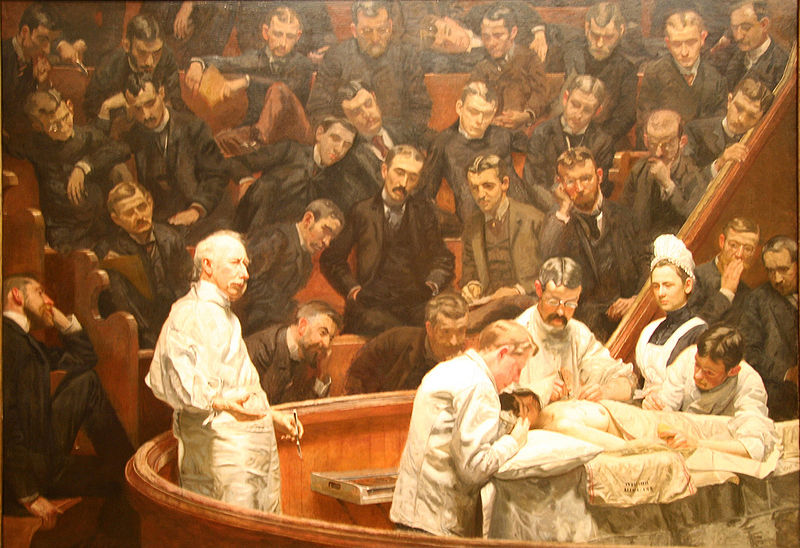
\includegraphics[height=.8\textheight ]{images/painting}\\
		\scriptsize The Agnew Clinic 1889 | Source: Thomas Eakins
	\end{center}

\end{frame}



\begin{frame}{Endoscopy (Definition)}

	\begin{myDefinition}
		\textit{Endoscopy} is derived from ancient Greek:
		\begin{center}
			endon $\equiv$ inside\\
			skopein $\equiv$ to see
		\end{center}
		\bigskip
		Endoscopy is often used in a medical environment to look inside a body for diagnosis or therapy. Minimally invasive procedures are daily performed on both animals and humans.
	\end{myDefinition}
\end{frame}



\begin{frame}{First Minimally Invasive Procedures}

	\begin{tabular}{lp{28em}}
		\textbf{1806}: & Philipp Bozzini engineers the first rigid endoscope using a candle as a light source \\
		\textbf{1855}: & Antonin J. Desormeaux replaced the candle in Bozzini's setup by a gas arc lamp       \\
	\end{tabular}

	\begin{center}
		\begin{tabular}{c c}
			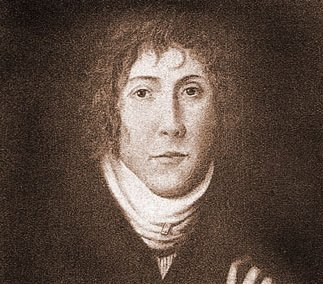
\includegraphics[height=.45\textheight ]{images/BozziniPhilip}        &
			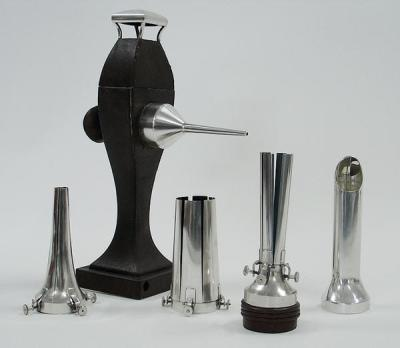
\includegraphics[height=.45\textheight ]{images/lichtleiter}            \\
			\scriptsize Philipp Bozzini | Source: American Urological Association &
			\scriptsize Lichtleiter | Source: Nitze-Leiter-Gesellschaft
		\end{tabular}
	\end{center}

\end{frame}




\begin{frame}{First Minimally Invasive Procedures}

	\begin{tabular}{lp{28em}}
		\textbf{1912}: & Hans Christian Jacobaeus uses endoscopic intervention to explore the abdomen and the thorax \\
		\textbf{1958}: & Basil Hirschowitz invents the first flexible endoscope                                      \\
		\textbf{2000}: & Capsule endoscopy is introduced
	\end{tabular}

	\begin{center}
		\begin{tabular}{c c c}
			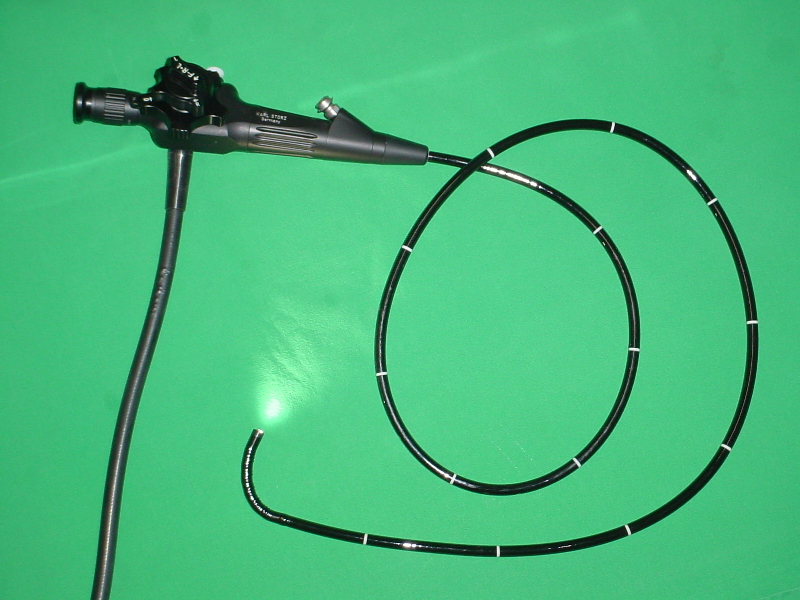
\includegraphics[height=.45\textheight ]{images/flexible} &
			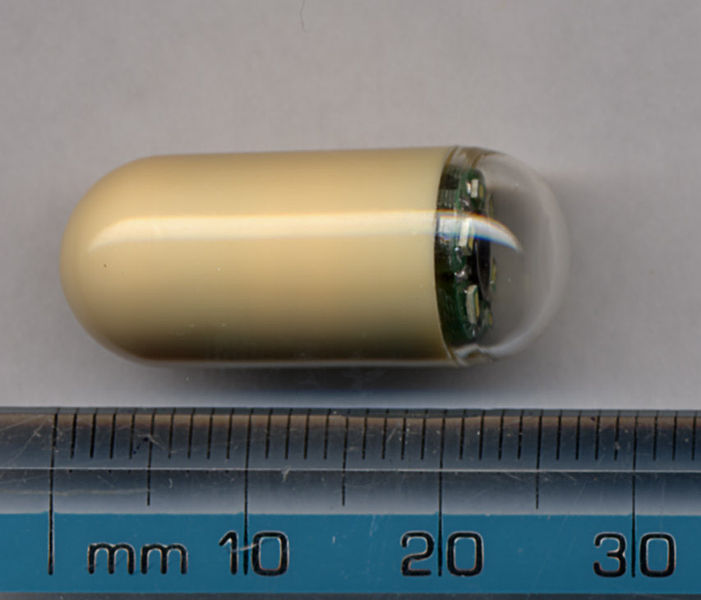
\includegraphics[height=.45\textheight ]{images/capsule}    \\
			\scriptsize Fiberskop | Source: Wikimedia Commons         &
			\scriptsize Capsule | Source: Wikimedia Commons
		\end{tabular}
	\end{center}

\end{frame}



\begin{frame}{Outline}
	\begin{itemize}
		\item History
		      \bolditem{} Setup
		\item Endoscopic Interventions
		\item NOTES
		\item 3-D Endoscopy
		\item Computer Assistance
		\item Future Trends
	\end{itemize}
\end{frame}

\begin{frame}[t]{Projection Models}
	Orthographic Projection


	\begin{columns}[c, onlytextwidth]
		\begin{column}{0.5\textwidth}
			\vspace{1.5cm}
			$$\left(\begin{array}{c}i_x\\i_y\end{array}\right) = \left(\begin{array}{ccc}1 &0 &0\\ 0&1&0\end{array}\right) \left(\begin{array}{c}x\\y\\z\end{array}\right)$$
			\vspace{1.5cm}
		\end{column}\begin{column}{0.5\textwidth}
			\begin{center}
				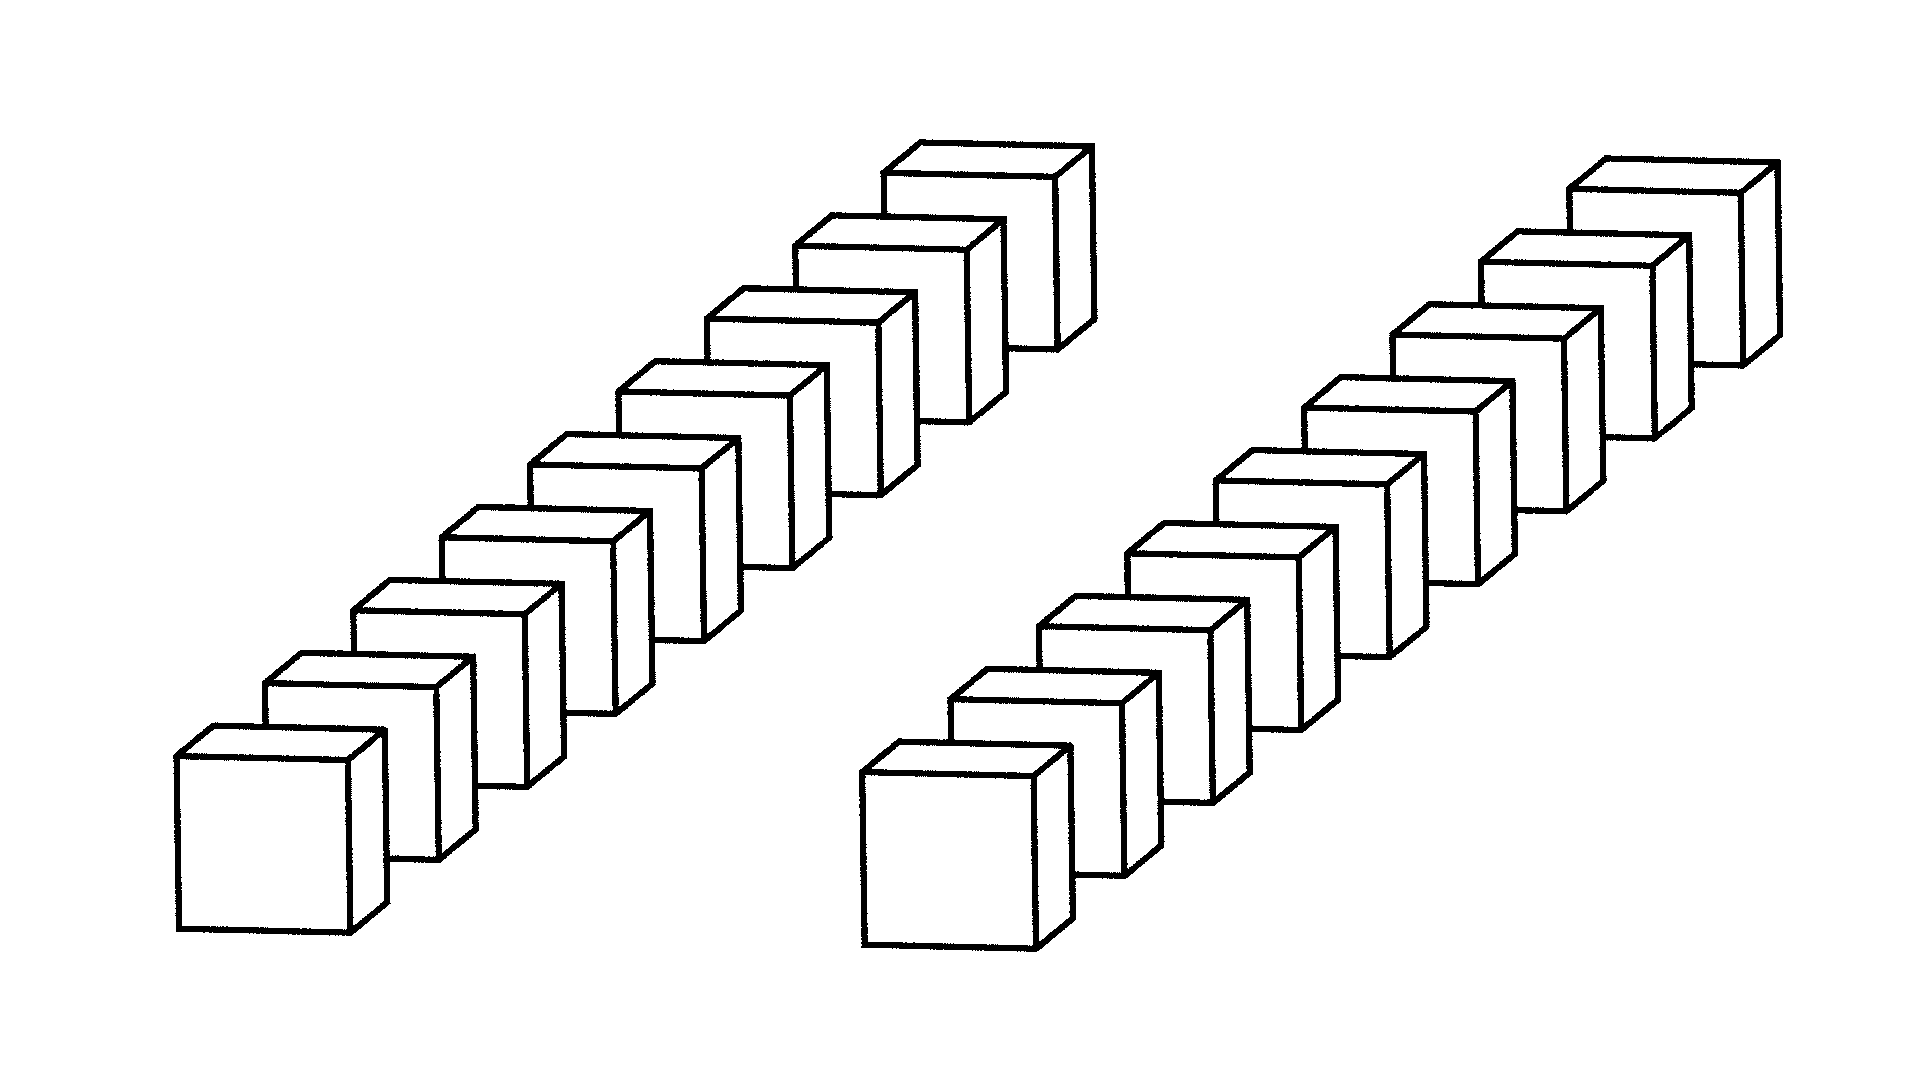
\includegraphics[width=1.1\textwidth]{images/orthographic.png}
			\end{center}
		\end{column}
	\end{columns}
	\begin{itemize}
		\item Neglects distance to screen
	\end{itemize}
\end{frame}


\begin{frame}[t]{Projection Models}
	Weak Perspective Projection
	\begin{columns}[c, onlytextwidth]
		\begin{column}{0.5\textwidth}
			\vspace{1.5cm}
			$$\left(\begin{array}{c}i_x\\i_y\end{array}\right) = \left(\begin{array}{ccc}k &0 &0\\ 0&k&0\end{array}\right) \left(\begin{array}{c}x\\y\\z\end{array}\right)$$
			\vspace{1.5cm}
		\end{column}\begin{column}{0.5\textwidth}
			\begin{figure}
				\begin{center}
					\only<1>{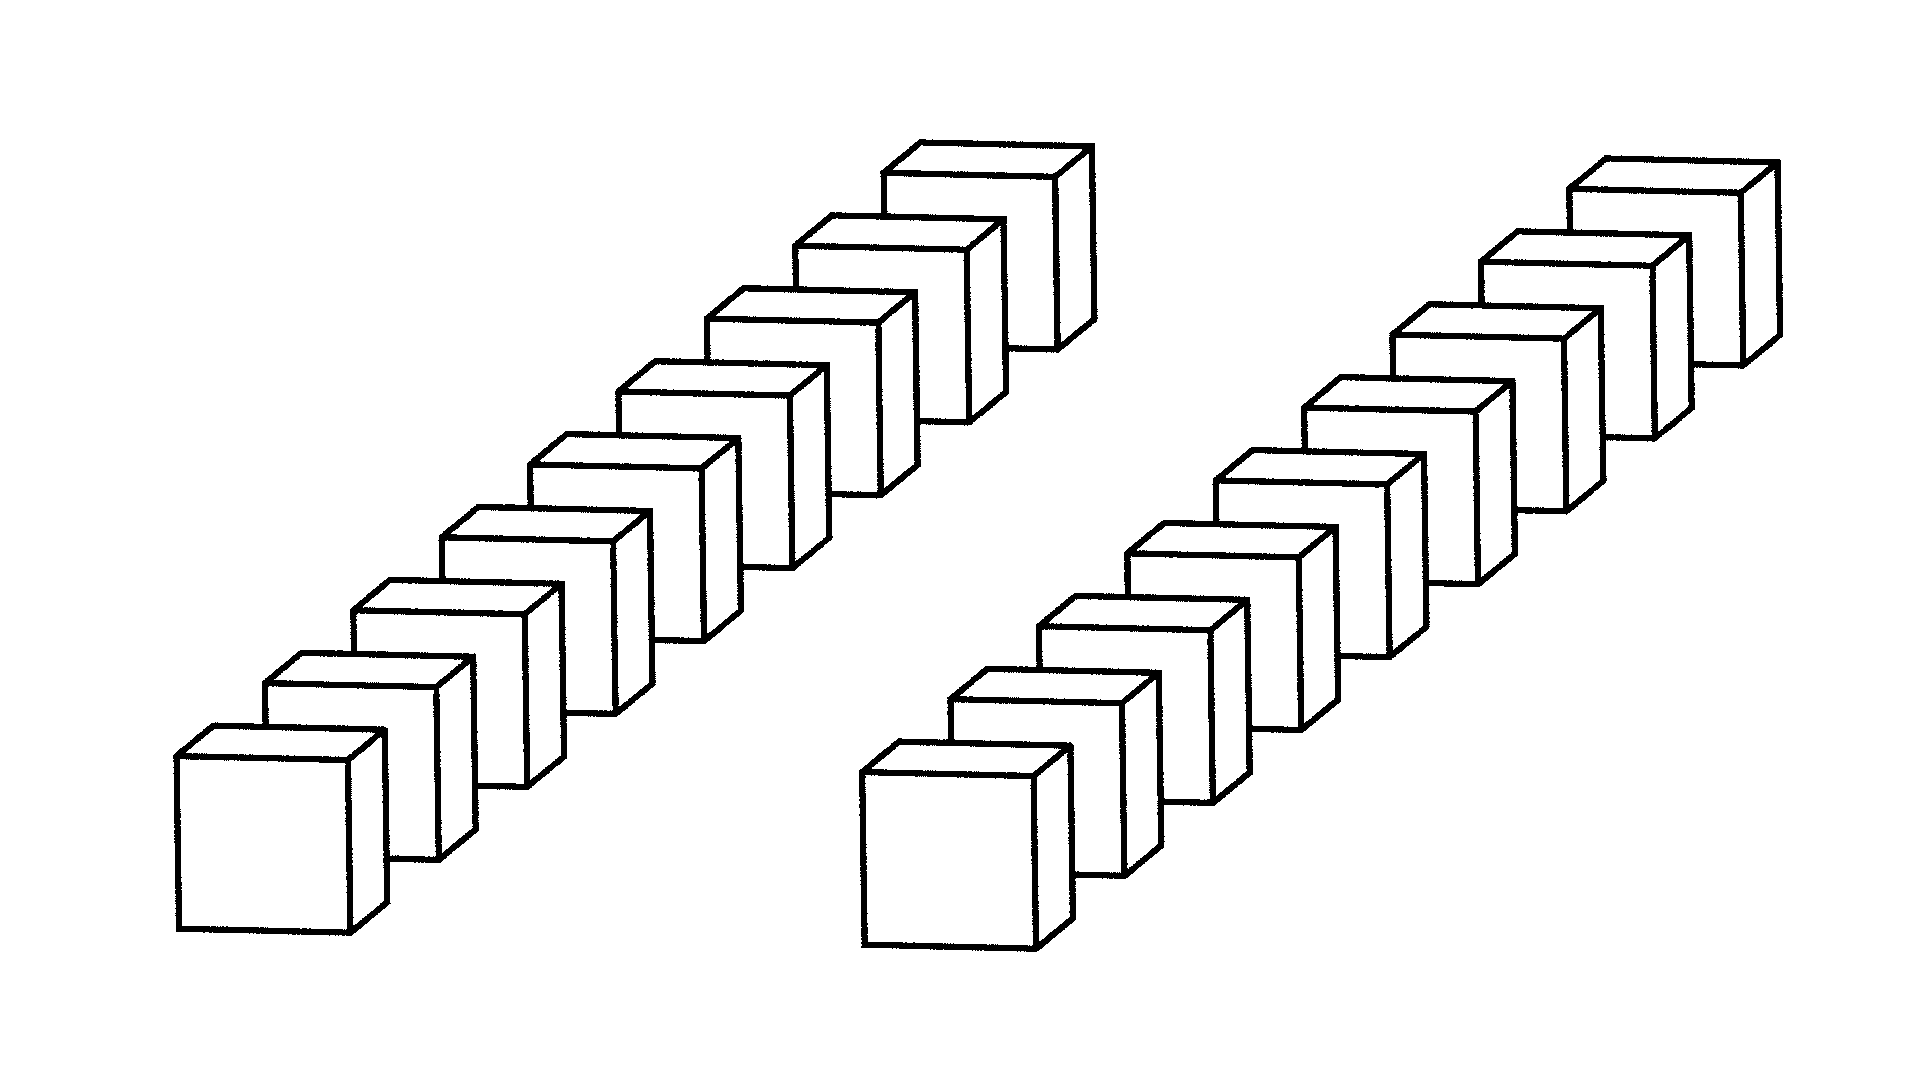
\includegraphics[width=0.9\textwidth]{images/orthographic.png}}
					\only<2>{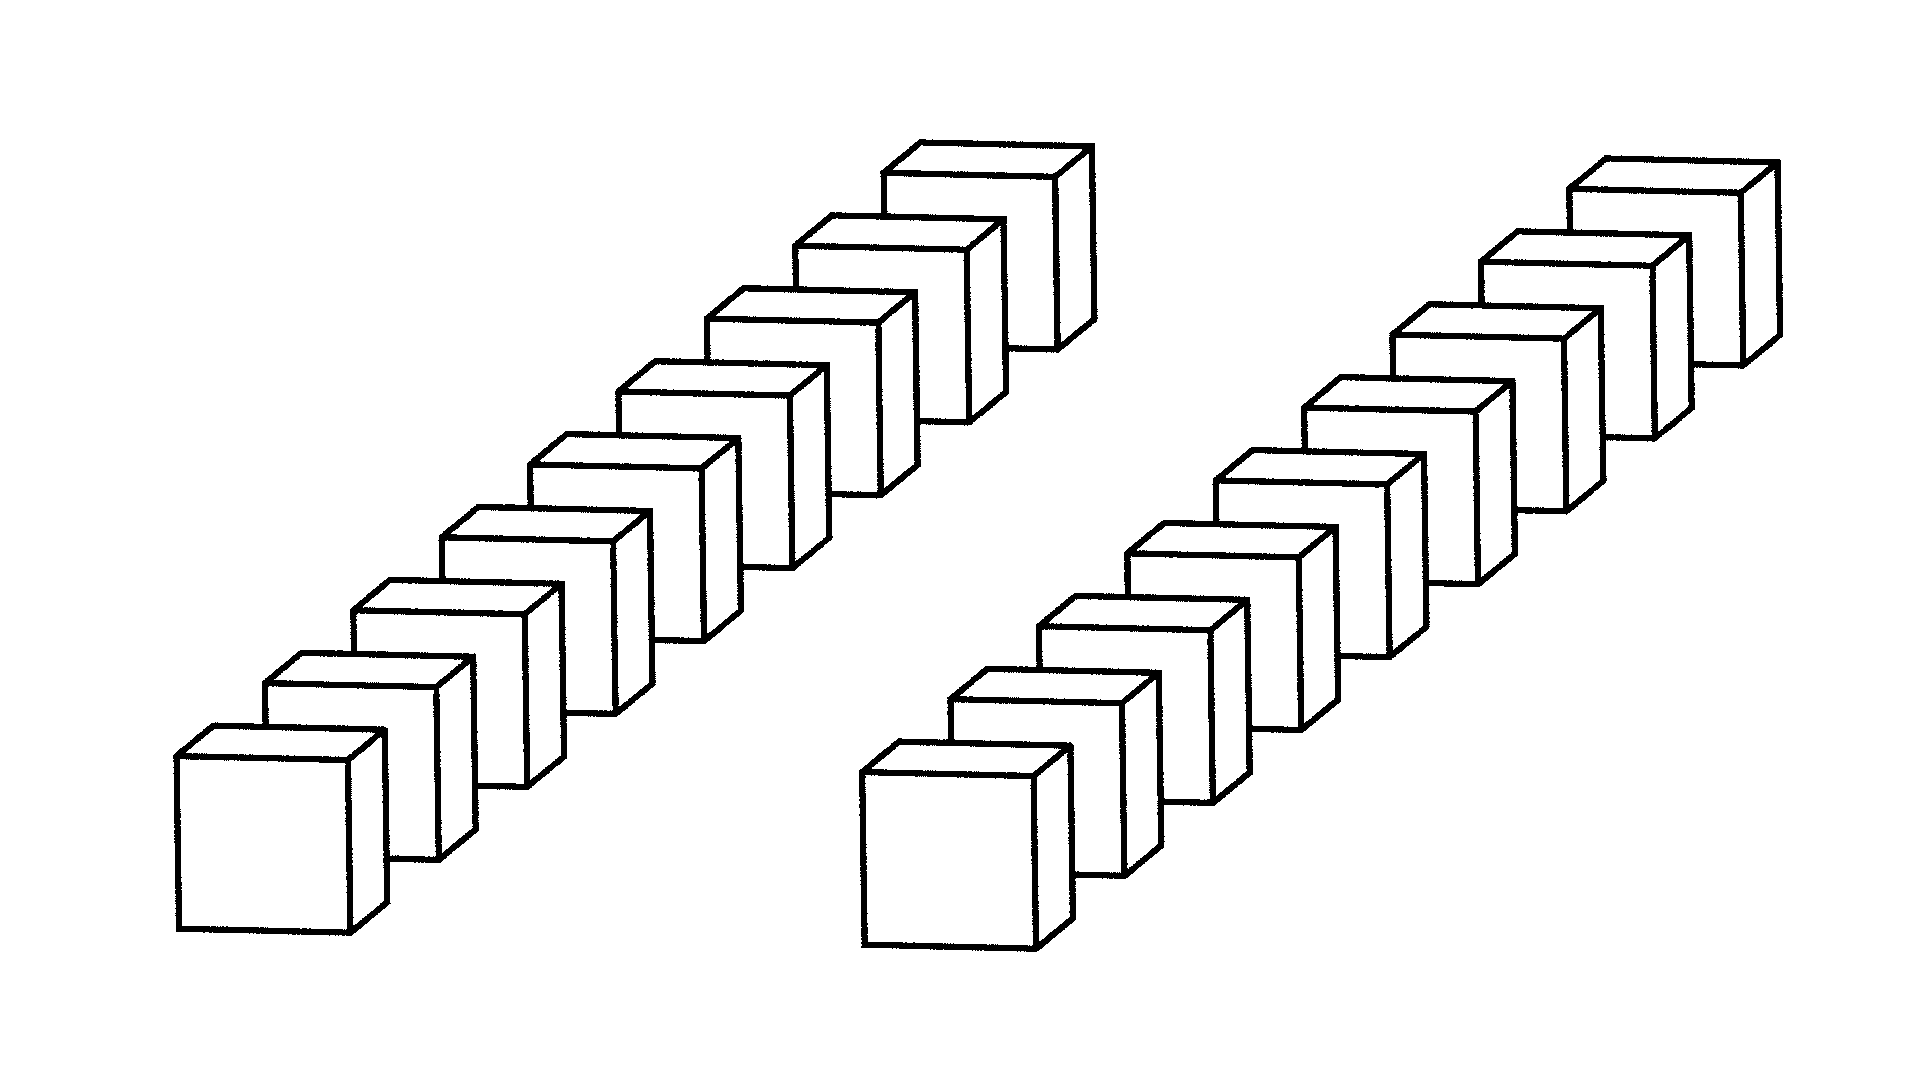
\includegraphics[width=0.7\textwidth]{images/orthographic.png}}
					\only<3>{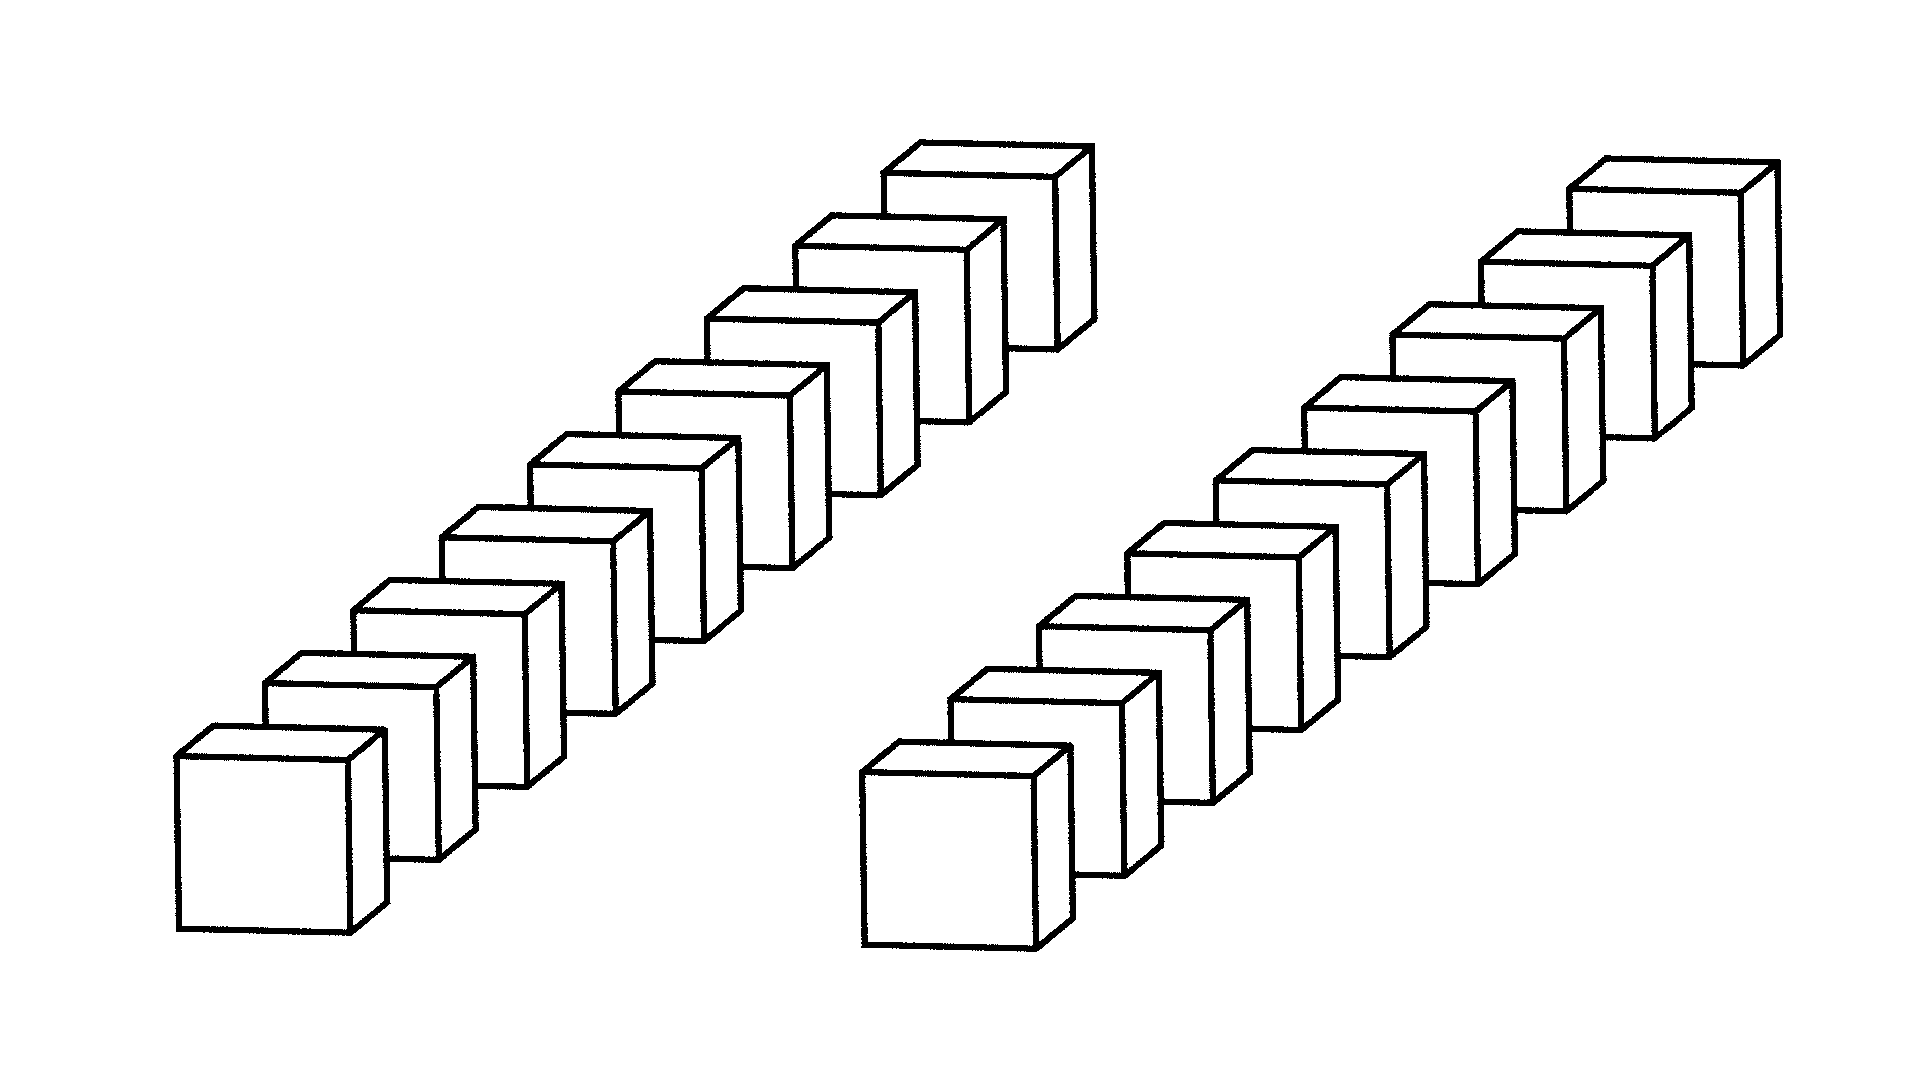
\includegraphics[width=0.5\textwidth]{images/orthographic.png}}
				\end{center}
			\end{figure}


		\end{column}
	\end{columns}
	\vspace{-1cm}
	\begin{columns}[c, onlytextwidth]
		\begin{column}{0.5\textwidth}
		\end{column}\begin{column}{0.5\textwidth}
		\begin{center}
			\scriptsize	
			\color{faublue}{
			Scaling by $k$
		}
		\end{center}
		\end{column}
	\end{columns}

	\begin{itemize}
		\item Introduces a fixed scaling $k$
		\item Scaling only accurate for objects in fixed distance
	\end{itemize}
\end{frame}

\begin{frame}[t]{Projection Models}
	Perspective Projection
	\begin{columns}[c, onlytextwidth]
		\begin{column}{0.5\textwidth}
			\vspace{1cm}
			$$\left(\begin{array}{c}i_x \\i_y\end{array}\right) =\left(\begin{array}{c} \frac{f\cdot x}{z} \\\frac{f\cdot y}{z}\end{array}\right) $$
			$$= \left(\begin{array}{ccc} ? &? &?\\ ?&?&?\end{array}\right) \left(\begin{array}{c}x\\y\\z\end{array}\right)$$
			\vspace{1cm}
		\end{column}\begin{column}{0.5\textwidth}
			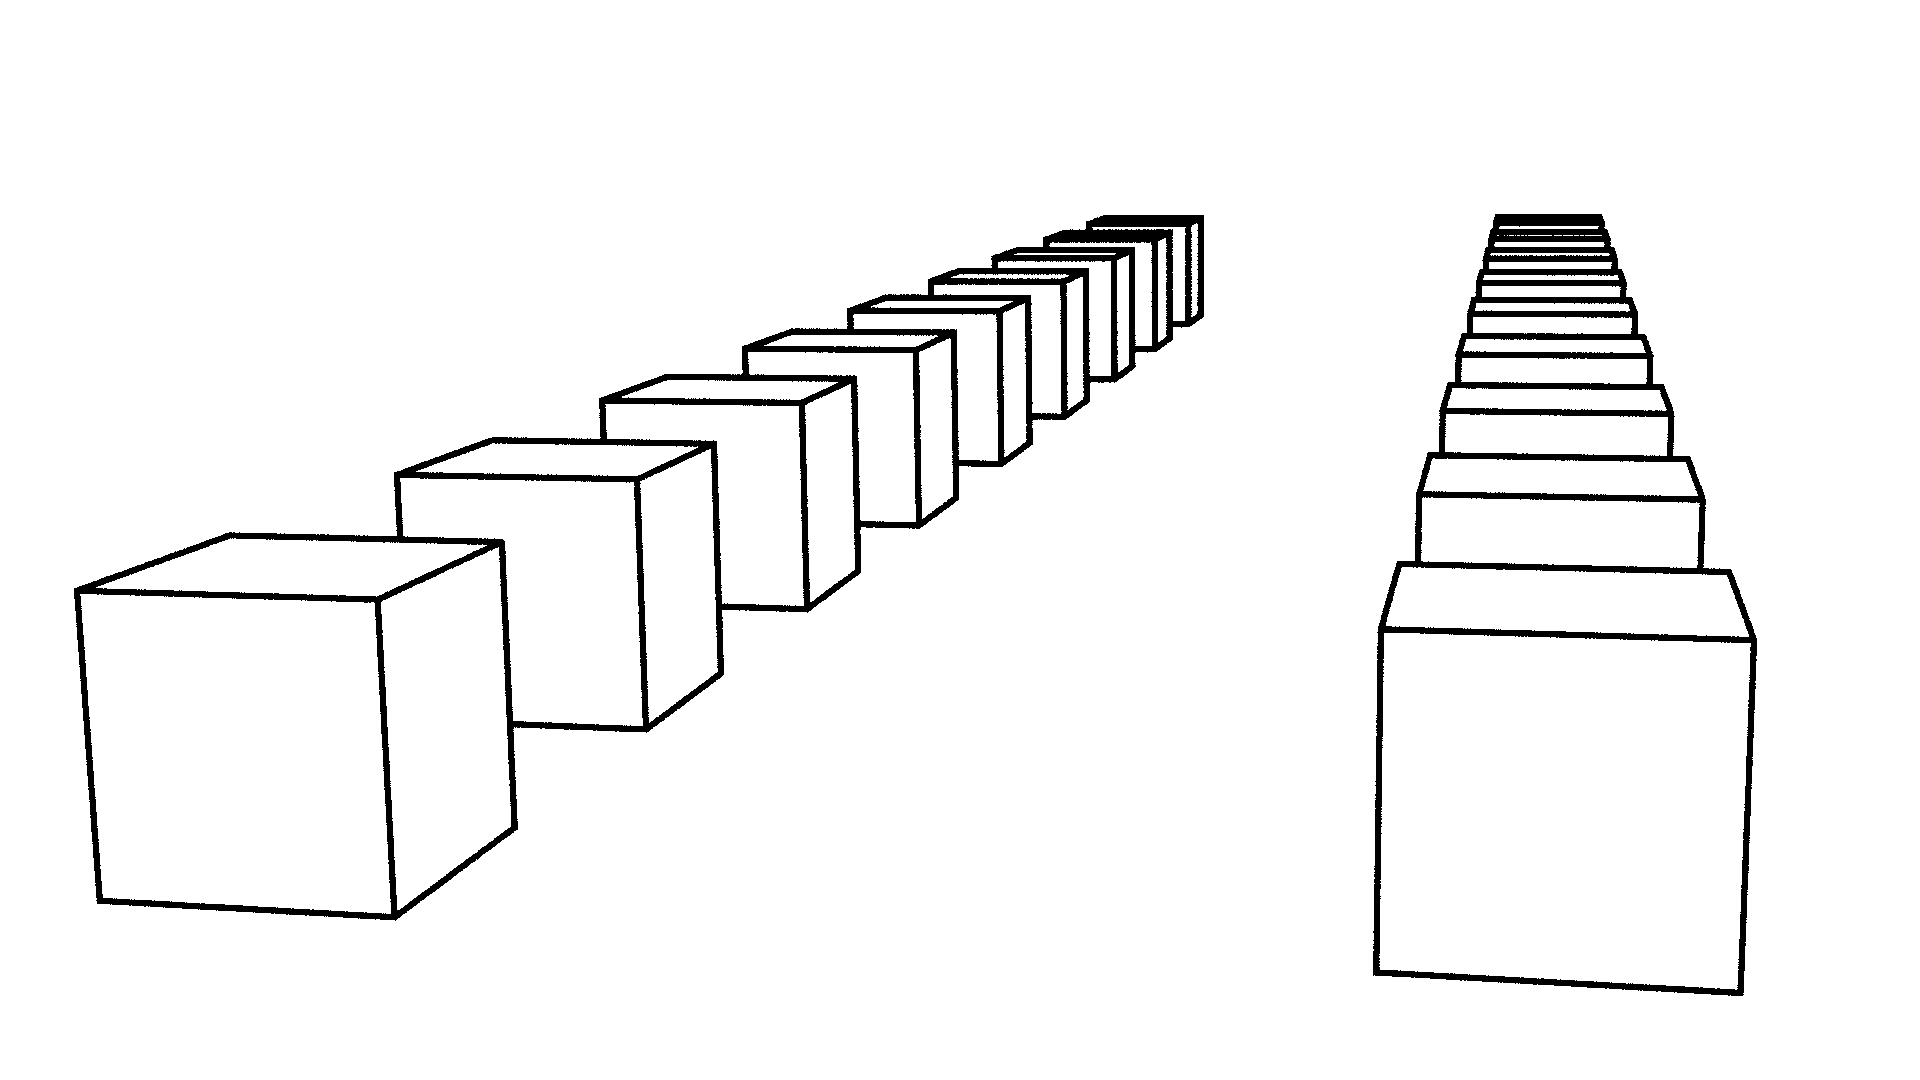
\includegraphics[width=\textwidth]{images/perspective.png}
		\end{column}
	\end{columns}

	\begin{itemize}
		\item Scaling depending on focal length $f$ and distance to screen $z$
		\item No longer a linear transform
	\end{itemize}
\end{frame}

\begin{frame}[t]{Projection Models}
	\begin{figure}[htpb]
		\centering

		\def\svgwidth{0.9\textwidth}
		\only<1>{\input{projection_color_1.pdf_tex}}%
		\only<2>{\input{projection_color_6.pdf_tex}}%
		\only<3>{\input{projection_color_3.pdf_tex}}%

	\end{figure}
	\begin{minipage}[c][2cm][c]{\textwidth}
		\only<1>{
			\begin{equation*}
				\left(\begin{array}{c}i_x\\i_y\end{array}\right) = \left(\begin{array}{ccc}1 &0 &0\\ 0&1&0\end{array}\right) \left(\begin{array}{c}x\\y\\z\end{array}\right)
			\end{equation*}
		}
		\only<2>{
			\begin{equation*}
				\left(\begin{array}{c}i_x\\i_y\end{array}\right) = \left(\begin{array}{ccc}k &0 &0\\ 0&k&0\end{array}\right) \left(\begin{array}{c}x\\y\\z\end{array}\right)
			\end{equation*}
		}
		\only<3>{
			\begin{equation*}
				\left(\begin{array}{c}i_x \\i_y\end{array}\right) =\left(\begin{array}{c} \frac{f\cdot x}{z} \\\frac{f\cdot y}{z}\end{array}\right)
				= \left(\begin{array}{ccc} ? &? &?\\ ?&?&?\end{array}\right) \left(\begin{array}{c}x\\y\\z\end{array}\right)
			\end{equation*}
		}
	\end{minipage}

\end{frame}

\begin{frame}[t]{Pinhole Camera Model}
	\begin{itemize}
		\item The pinhole camera model generates an image on the opposing side
		\item The image is scaled and upside-down
	\end{itemize}
	\begin{figure}
		\centering
		\begin{tikzpicture}[scale=1, transform shape]
			\node (dsa) []  {\reflectbox{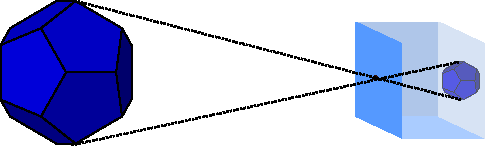
\includegraphics[width=0.9\linewidth]{images/pinhole_new.pdf}
				}};
			\node (image) [ align=center,anchor=north] at (-4.7,-1.8) {Flipped\\Image};
			\node (fp) [anchor=north,align=center] at (-2.9,-1.8) {Focal\\ Point};
			\node (obj) [anchor=north] at (4,-1.8) {Object};


		\end{tikzpicture}
	\end{figure}
\end{frame}

\begin{frame}[t]{Virtual Screen Model}

	\begin{itemize}
		\item The pinhole camera model can be simplified by introducing a virtual screen
		\item The virtual screen avoids flipping the image
	\end{itemize}

	\begin{figure}
		\centering
		\begin{tikzpicture}[scale=1, transform shape]
			\node (dsa) []  {\reflectbox{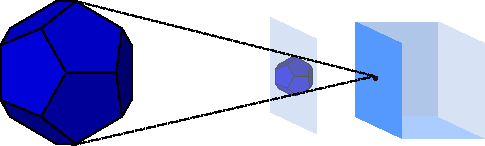
\includegraphics[width=0.9\linewidth]{images/pinhole_with_virtual_screen.pdf}
				}};
			\node (image) [ align=center,anchor=north] at (-1,-1.8) {Virtual\\Screen};
			\node (fp) [anchor=north,align=center] at (-2.85,-1.8) {Focal\\ Point};
			\node (fpmark) [coordinate, above=1.5cm of fp] {};
			\node (obj) [anchor=north] at (4,-1.8) {Object};

			%\path[draw=black,dashed, line width=0.4mm] (fp) -- (fpmark) node[midway, above right] {};

		\end{tikzpicture}


	\end{figure}
\end{frame}

\begin{frame}[c]{Virtual Screen Model}

	\begin{itemize}
		\item The pinhole camera model can be simplified by introducing a virtual screen
		\item The virtual screen avoids flipping the image
	\end{itemize}

	\begin{figure}
		\centering
		\begin{tikzpicture}[scale=1, transform shape]
			\node (dsa) []  {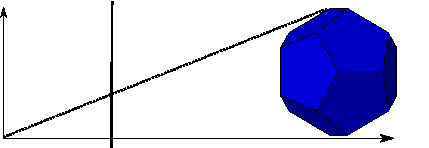
\includegraphics[width=0.9\linewidth]{images/virtualscreen.pdf}};
			\node (image) [ align=center,anchor=north] at (-2.5,-1.8) {Virtual\\Screen};
			\node (fp) [anchor=north,align=center] at (-5.2,-1.8) {Focal\\ Point};
			\node (fpmark) [coordinate, above=1.5cm of fp] {};
			\node (obj) [anchor=north] at (3.3,-1.8) {Object};

			%\path[draw=black,dashed, line width=0.4mm] (fp) -- (fpmark) node[midway, above right] {};

		\end{tikzpicture}


	\end{figure}
\end{frame}

\begin{frame}{Rigid Endoscope}

	\begin{center}
		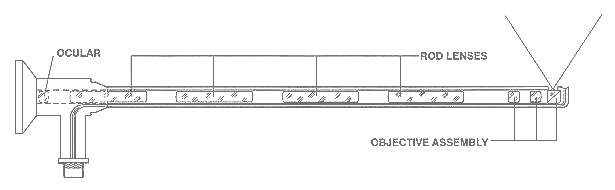
\includegraphics[height=.45\textheight ]{images/rigidSketch}\\
		\scriptsize Rigid Endoscope | Source: Imaginis
	\end{center}

\end{frame}



\begin{frame}{Flexible Endoscope}

	\begin{center}
		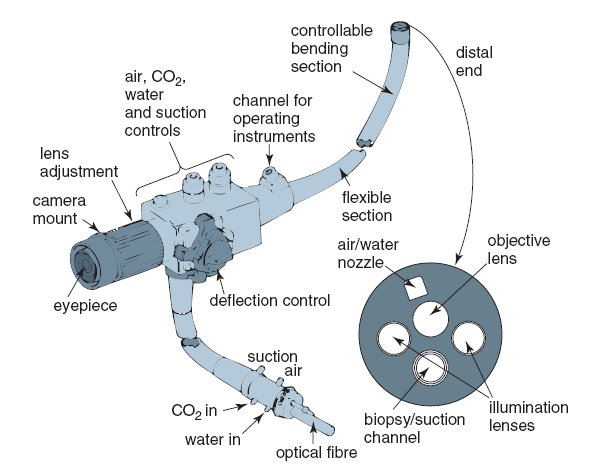
\includegraphics[height=.8\textheight ]{images/flexibleSketch}\\
		\scriptsize Flexible Endoscope | Source: Jacaranda Physics 1
	\end{center}

\end{frame}



\begin{frame}{Trocars}

	\begin{center}
		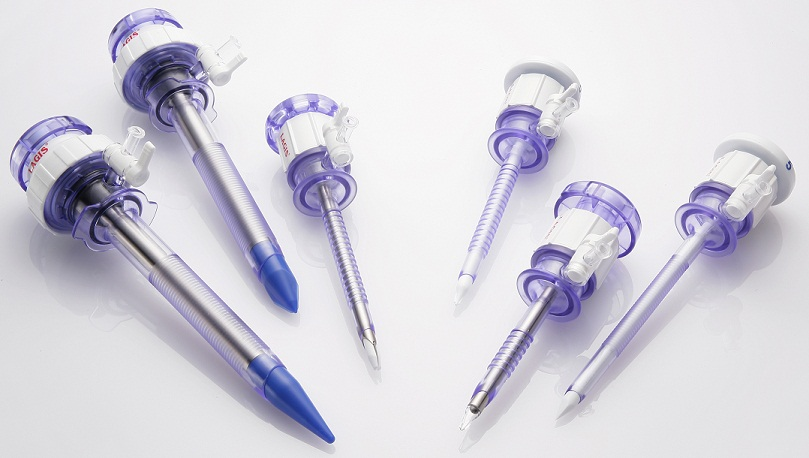
\includegraphics[height=.8\textheight ]{images/trocars}\\
		\scriptsize Different Trocars | Source: LAGIS
	\end{center}

\end{frame}



\begin{frame}{Tools}

	\begin{center}
		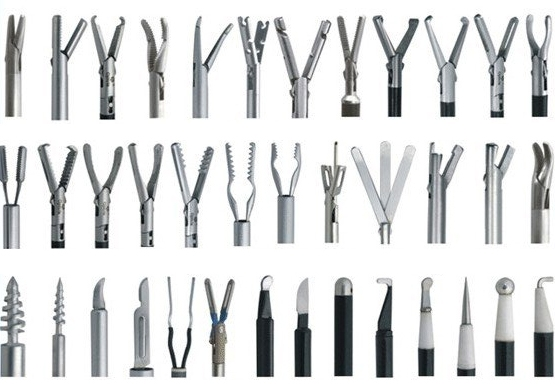
\includegraphics[height=.8\textheight ]{images/tools}\\
		\scriptsize Different Laparoscopic Tools | Source: Hangzhou OPTCLA Medical Instrument Co., Ltd.
	\end{center}

\end{frame}



\begin{frame}{Outline}
	\begin{itemize}
		\item History
		\item Setup
		      \bolditem{} Endoscopic Interventions
		\item NOTES
		\item 3-D Endoscopy
		\item Computer Assistance
		\item Future Trends
	\end{itemize}
\end{frame}



\begin{frame}{Endoscopy}
	\textbf{Advantages compared to open surgery:}
	\begin{itemize}
		\item[+] less operative trauma
		\item[+] only small scars
		\item[+] faster recovery time
		\item[+] shorter hospital stays
	\end{itemize}
	\vspace{1em}
	\textbf{Disadvantages compared to open surgery:}
	\begin{itemize}
		\item[-] loss of intuitive orientation
		\item[-] loss of sense for metric dimensions
	\end{itemize}

\end{frame}



\begin{frame}{Endoscopic Interventions}

	\begin{tabular}{lp{23em}}
		\textbf{Arthroscopy}:  & examination of joints                                                       \\
		\textbf{Bronchoscopy}: & examination of the trachea and lung (e.g. tubercolosis, tumor...)           \\
		\textbf{Colonoscopy}:  & examination of the colon (e.g. polyps, ulceration ...)                      \\
		\textbf{Cystoscopy}:   & examination of the urinary tract                                            \\
		\textbf{Gastroscopy}:  & examination of the esophagus, stomach, duodenum (e.g. ulcers  or bleedings) \\
		\textbf{Laparoscopy}:  & examination of the abdominal organs                                         \\
		\textbf{Rhinoscopy}:   & examination of the nose                                                     \\
		\textbf{Otoscopy}:     & examination of the ears                                                     \\
		\textbf{Proctoscopy}:  & examination of the rectum and sigmoid colon
	\end{tabular}

\end{frame}



%\begin{frame}{Laparoscopy Sketch}

%\begin{center}
%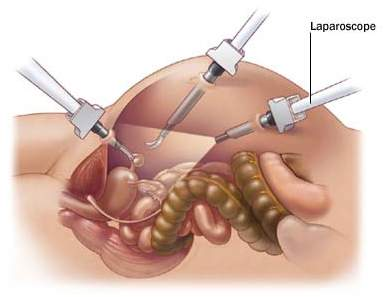
\includegraphics[height=.8\textheight ]{images/laparoscopy}\\
%\scriptsize Laparoscopic oophorectomy | Source: Mayo Foundation for Medical Education and Research
%\end{center}

%\end{frame}



%\begin{frame}{Gallbladder Operation}

%\begin{center}
%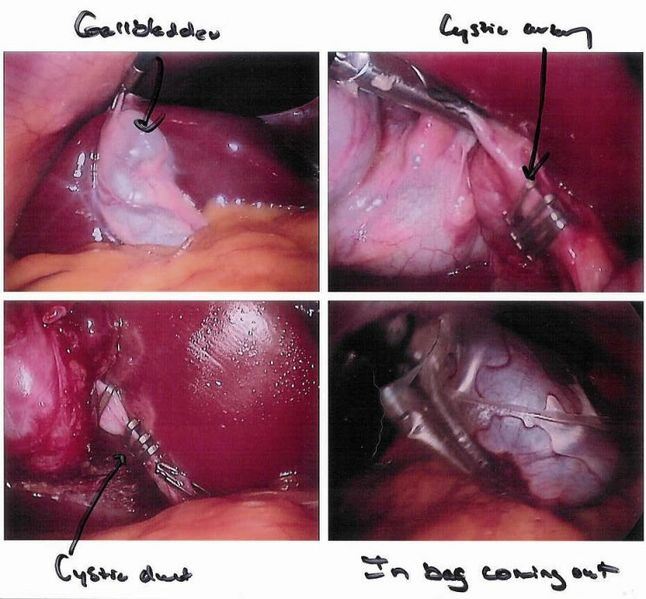
\includegraphics[height=.8\textheight ]{images/Gallbladder}\\
%\scriptsize Gallbladder, cystic artery, cystic duct, In bag | Source: Wikimedia Commons
%\end{center}

%\end{frame}



\begin{frame}{Laparoscopy}

	\begin{itemize}
		\bolditem Preparation:
		\begin{enumerate}
			\item Stop taking certain medicine (e.g. aspirin...)
			\item Do not drink for 6-12 hours
			\item Remove jewelry and clothes
		\end{enumerate}
		\bolditem Procedure
		\bolditem Recovery
	\end{itemize}

\end{frame}



\begin{frame}{Laparoscopy}

	\begin{itemize}
		\bolditem Preparation
		\bolditem Procedure:
		\begin{enumerate}
			\item Several sensors will monitor the patients health
			\item Use of anesthesia
			\item Surgical site will be cleaned
			\item First small cut will be made
			\item Inflate abdomen with $CO_2$
			\item Additional cuts may be performed
			\item Laparoscope and instruments are inserted
			\item Procedure is performed
			\item Incisions are closed with stitched
		\end{enumerate}
		\bolditem Recovery
	\end{itemize}

\end{frame}



\begin{frame}{Laparoscopy}

	\begin{itemize}
		\bolditem{} Preparation
		\bolditem{} Procedure
		\bolditem{} Recovery:
		\begin{enumerate}
			\item Patient is instructed how to keep the wound clean
			\item Setup date for follow-up appointment (e.g. to have stitches removed)
			\item Some $CO_2$ might remain and will be absorbed by our body
			\item Recovery may take up to 12 weeks
		\end{enumerate}
	\end{itemize}

\end{frame}



\begin{frame}{Outline}
	\begin{itemize}
		\item History
		\item Setup
		\item Endoscopic Interventions
		      \bolditem NOTES
		\item 3-D Endoscopy
		\item Computer Assistance
		\item Future Trends
	\end{itemize}
\end{frame}



\begin{frame}{NOTES (Definition)}

	\begin{myDefinition}
		\begin{center}
			\textit{NOTES} $\equiv$ \textbf{N}atural \textbf{O}rifice \textbf{T}ransluminal \textbf{E}ndoscopic \textbf{S}urgery
		\end{center}

		It means that it is a "scarless" procedure through a natural orifice (e.g. mouth, anus, etc.). Incisions will only be performed internal (e.g. stomach, colon, etc.).

		Still in an early experimental stage but already allowed to be performed on humans. In practice basically performed in hybrid techniques, where an additional access is necessary (e.g. through the navel).
	\end{myDefinition}
\end{frame}



%\begin{frame}
%\frametitle{NOTES (History)}
%\begin{itemize}
%	\item First described for animals by Dr. Anthony Kalloo et al. at Johns Hopkins University
%	\item June 25, 2007: \textbf{USGI Medical} announces first NOTES transgastric cholecystectomy procedures
%	\item January 29, 2009: Healthy kidney was removed through vagina for organ donation (by Johns Hopkins University)
%	\item until April, 2013: 2784 NOTES procedures were performed in Germany (2696 with transvaginal hybrid technique)
%\end{itemize}
%\end{frame}



\begin{frame}{NOTES}

	\textbf{Advantages compared to conventional endoscopy:}
	\begin{itemize}
		\item[+] less anesthetic (due to less pain through stomach)
		\item[+] shorter recovery time
		\item[+] no external scars
	\end{itemize}
	\vspace{1em}
	\textbf{Disadvantages compared to conventional endoscopy:}
	\begin{itemize}
		\item[-] unsterile access points
		\item[-] endoscopes must be very flexible (no stable abutment)
	\end{itemize}

\end{frame}

\begin{frame}{Confocal Laser Endomicroscopy (CLE)}
	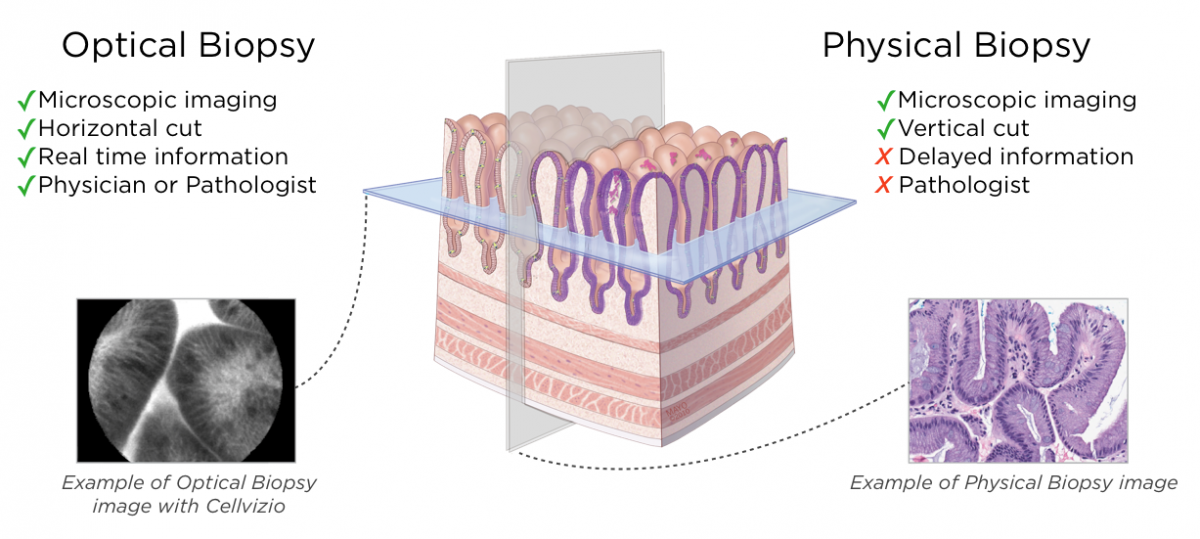
\includegraphics[width=0.8\textwidth]{img2/basics_optical_physical.png}

	CLE allows real time visualization of epithel layer in vivo!
\end{frame}

\begin{frame}{Confocal Laser Endomicroscopy}
	Very high magnification \& resolution images of mucosal layer of the GI tract

	\begin{columns}[T]
		\begin{column}{0.4\textwidth}
			\begin{tabular}{ll}
				Depth ($\mu m$)         & 55-65 \\
				Field of view ($\mu m$) & 240   \\
				Imaging rate (fps)      & 12.8  \\
			\end{tabular}
		\end{column}
		\begin{column}{0.5\textwidth}
			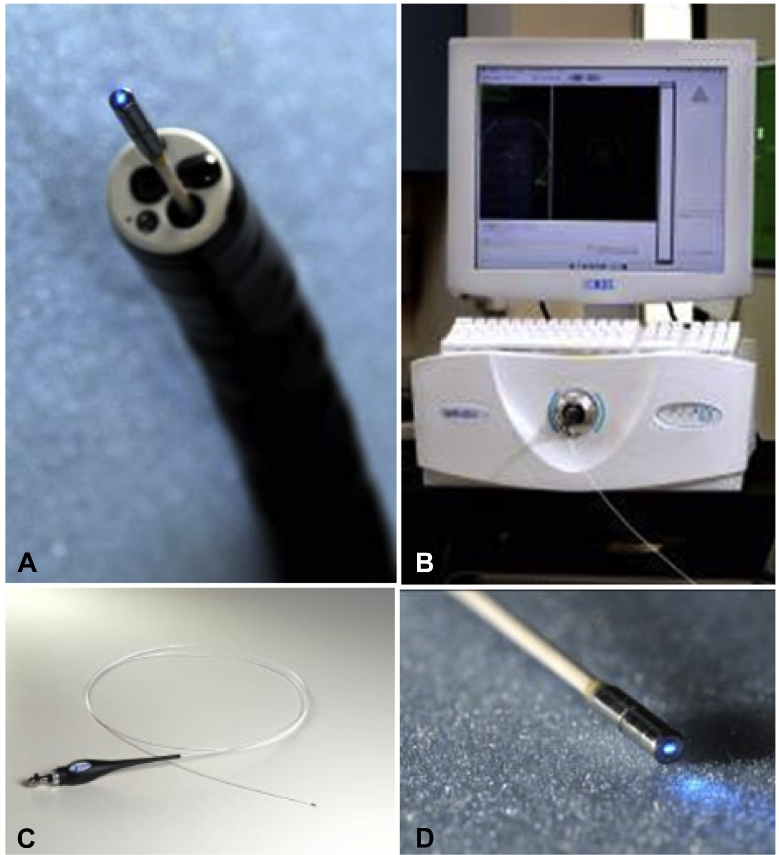
\includegraphics[height=0.7\textheight]{img2/cle_system.png}

			\tiny{Source: Confocal Laser Endomicroscopy, American Society for Gastrointestinal Endoscopym, 80(6), 2014}
		\end{column}
	\end{columns}
\end{frame}
\begin{frame}{Confocal Laser Endomiscroscopy}

	%				\begin{columns}[T]
	%		\begin{column}{0.4\textwidth}
	\begin{itemize}
		%			\item based on tissue illumination w.\ a low-power laser
		%				with subsequent detection of the fluorescence of light reflected from
		%				the tissue through a pinholeo
		\item Each fiber collects the emitted light of the fluorophores at focus point, while ignoring
		      light out of focus and propagate it back to a mono-pixel photodetector
		\item 30\,000 glass fibers are combined to a fiber
		      bundle
		      %			\item every fiber can focus a certain point in the specimen
	\end{itemize}
	%		\end{column}
	%		\begin{column}{0.5\textwidth}
	%		\includegraphics[width=\textwidth]{img2/conf_principle.png}
	%		\tiny{Source: wiki-commons}

	%		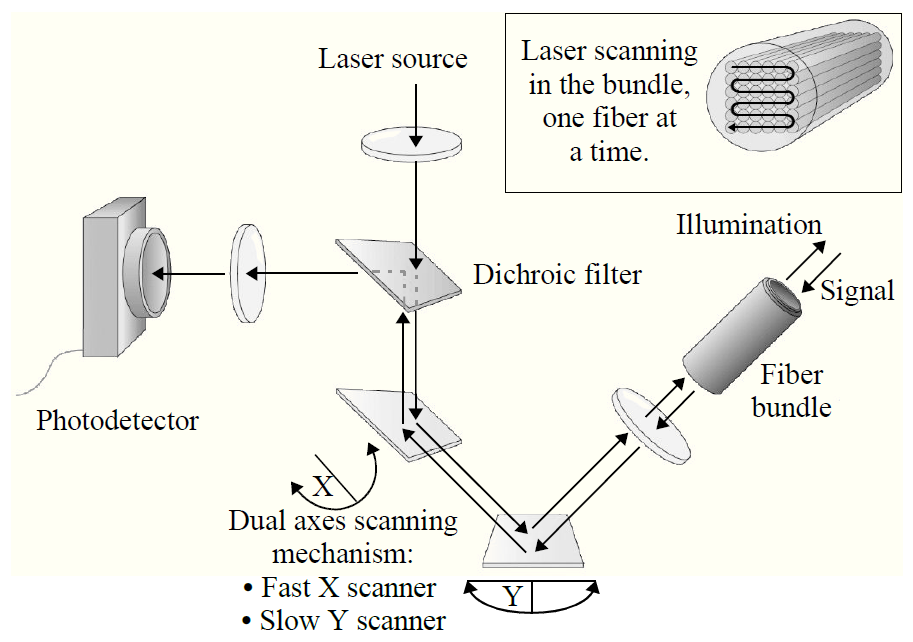
\includegraphics[width=\textwidth]{img2/pcle.png}
	\begin{center}
		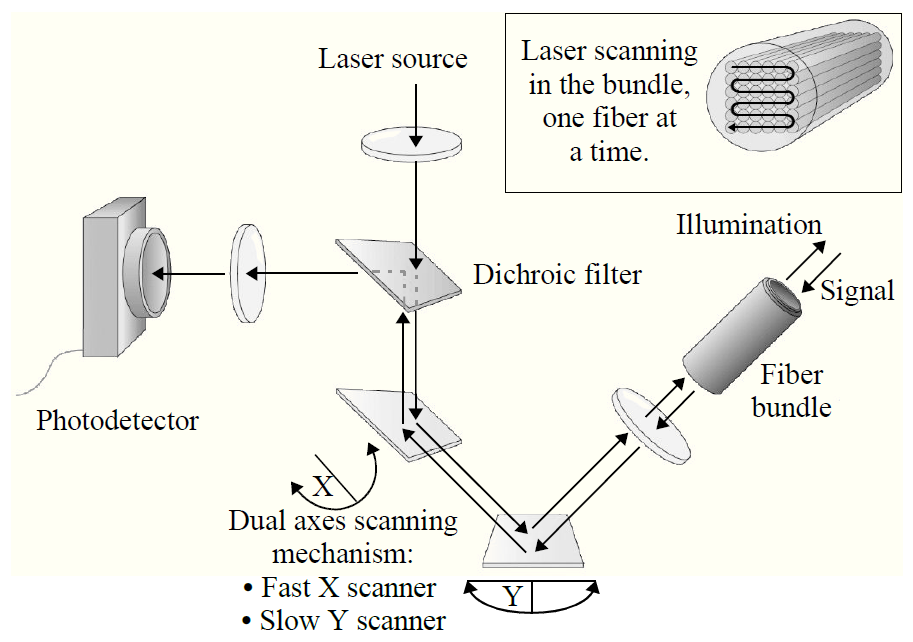
\includegraphics[height=0.6\textheight]{img2/pcle.png}

		\tiny{Souce: Abrat and Masters. Endoscopic Confocal Microscopy Moves into the
			Clinic, Biophotonics International, Nov 2006.}
	\end{center}
	\normalsize

	%	\end{column}
	%\end{columns}
\end{frame}
%\begin{frame}
%\frametitle{Hybrid NOTES}
%
%\begin{center}
%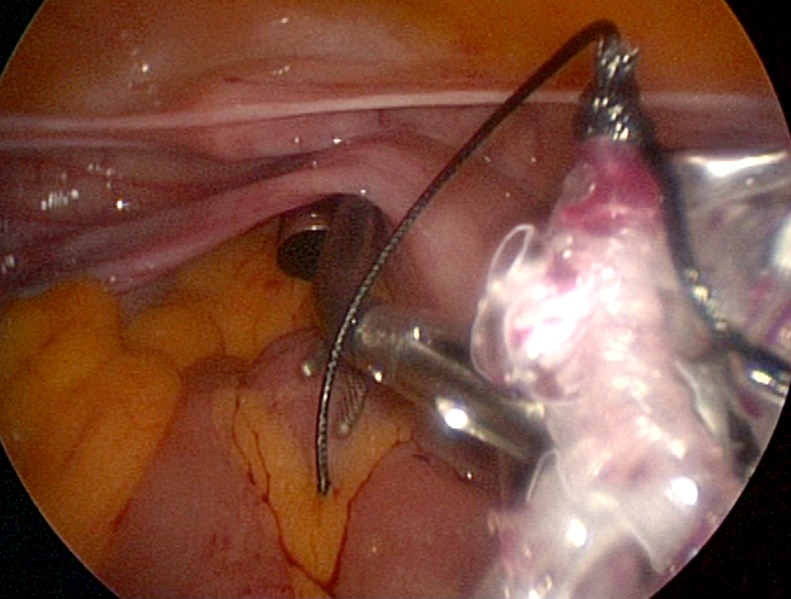
\includegraphics[height=.8\textheight ]{images/hybridNotes}\\
%\scriptsize Bag removal after gastric resection | Source: Wikimedia Commons
%\end{center}
%
%\end{frame}

\begin{frame}{Background Carcinogenesis}
	Development stages of oral cancer

	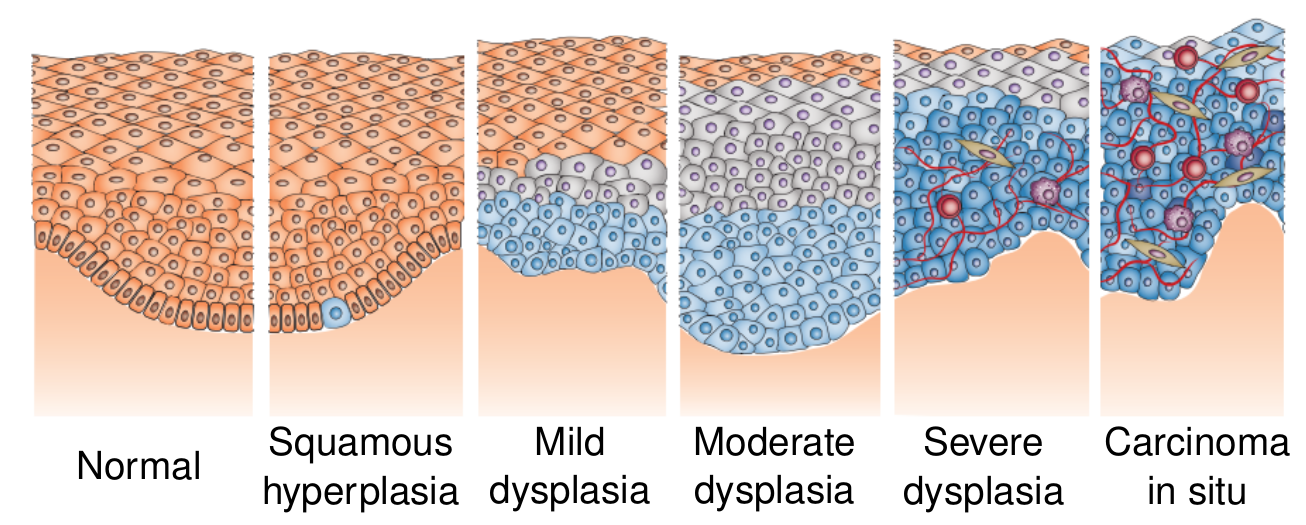
\includegraphics[width=0.9\textwidth]{img2/cancer_states.png}
\end{frame}

\begin{frame}{Examples}
	\begin{columns}[T]
		\begin{column}{0.45\textwidth}
			\centering
			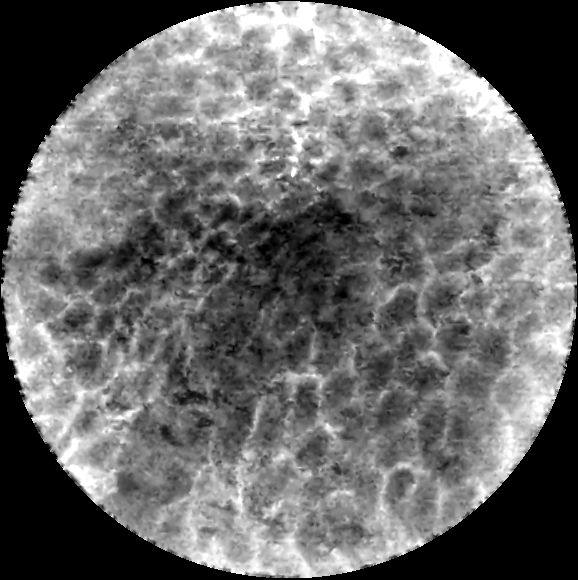
\includegraphics[height=0.75\textheight]{img2/healthy.png}

			Healty
		\end{column}%
		\begin{column}{0.45\textwidth}
			\centering
			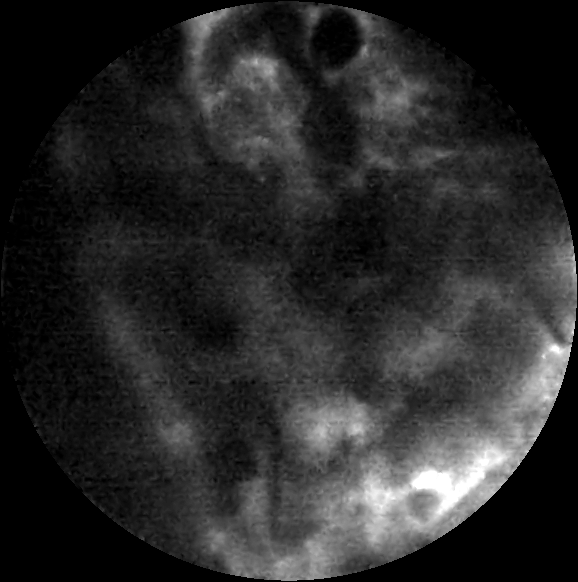
\includegraphics[height=0.75\textheight]{img2/carcinoma.png}

			Carcinoma
		\end{column}
	\end{columns}
\end{frame}

\begin{frame}{Outline}
	\begin{itemize}
		\item History
		\item Setup
		\item Endoscopic Interventions
		\item NOTES
		      \bolditem 3-D Endoscopy
		\item Computer Assistance
		\item Future Trends
	\end{itemize}
\end{frame}



\begin{frame}{3-D Endoscopy (Definition)}

	\begin{myDefinition}
		\textit{3-D Endoscopy} describes a technique to acquire metric range data about the surgical site within an endoscopic intervention. Range data delivers topographic information about the observed scene. It can be acquired using different techniques, e.g. stereo vision, structured light, Time-of-Flight.

		Most popular and commercially available systems are based on stereo vision similar to the human depth estimation.
	\end{myDefinition}
\end{frame}



\begin{frame}{3-D Endoscopy}

	\textbf{Advantages:}
	\begin{itemize}
		\item[+] allows metric measurements
		\item[+] mesh representation for intuitive visualization
		\item[+] collision avoidance (for computer guidance)
	\end{itemize}
	\vspace{1em}
	\textbf{Disadvantages:}
	\begin{itemize}
		\item[-] early scientific stage
		\item[-] all suffer from specular highlights
		\item[-] often unpopular for surgeons
	\end{itemize}

\end{frame}



\begin{frame}{Stereo Endoscopy}

	\begin{center}
		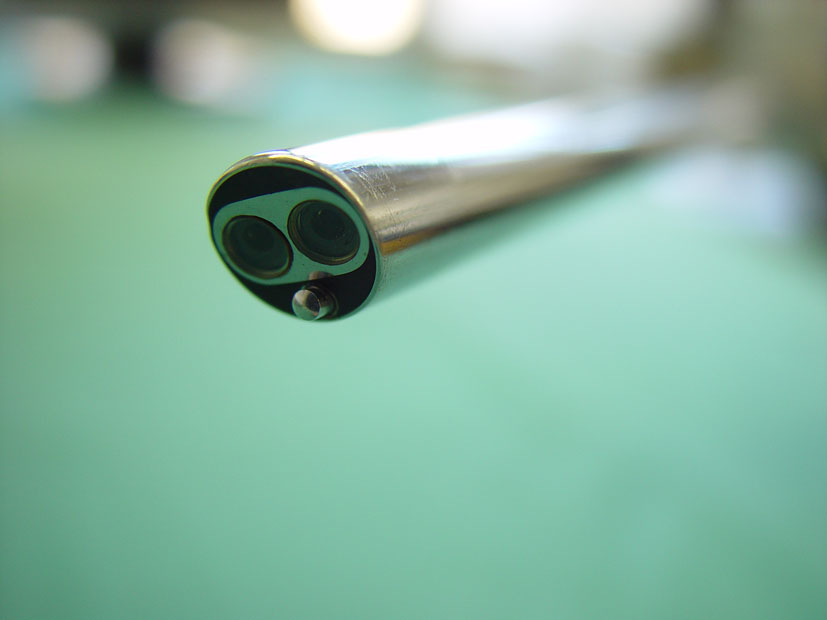
\includegraphics[height=.8\textheight ]{images/stereo}\\
		\scriptsize Stereo endoscope | Source: KIT
	\end{center}

\end{frame}



\begin{frame}{Stereo Endoscopy}

	\begin{center}
		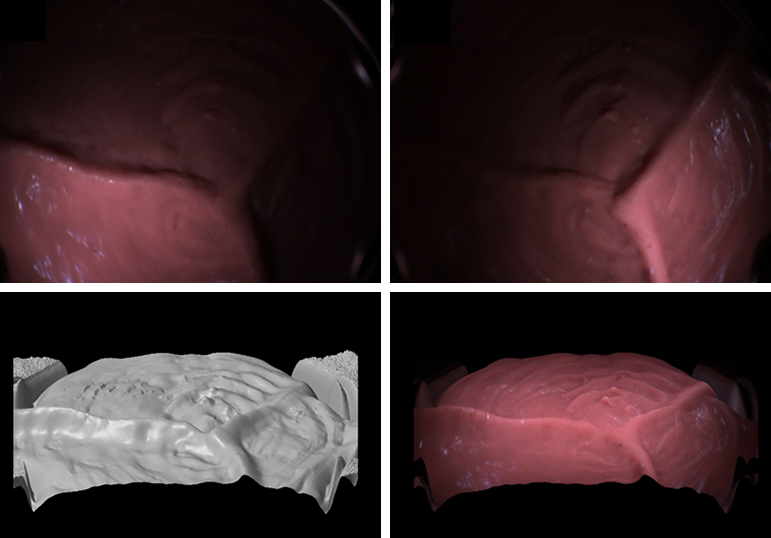
\includegraphics[height=.8\textheight ]{images/stereo1}\\
		\scriptsize Stereo endoscope data | Source:  "Photometric stereo endoscopy"
	\end{center}

\end{frame}



\begin{frame}{Stereo Endoscopy}

	\textbf{Advantages:}
	\begin{itemize}
		\item[+] HD endoscopes available
		\item[+] certified and commercially available
		\item[+] high range data accuracy
		\item[+] RGB and range information
	\end{itemize}
	\vspace{1em}
	\textbf{Disadvantages:}
	\begin{itemize}
		\item[-] range quality and range image resolution depends on texture
		\item[-] computational expensive feature matching
	\end{itemize}

\end{frame}



\begin{frame}{Structured Light Endoscopy}

	\begin{center}
		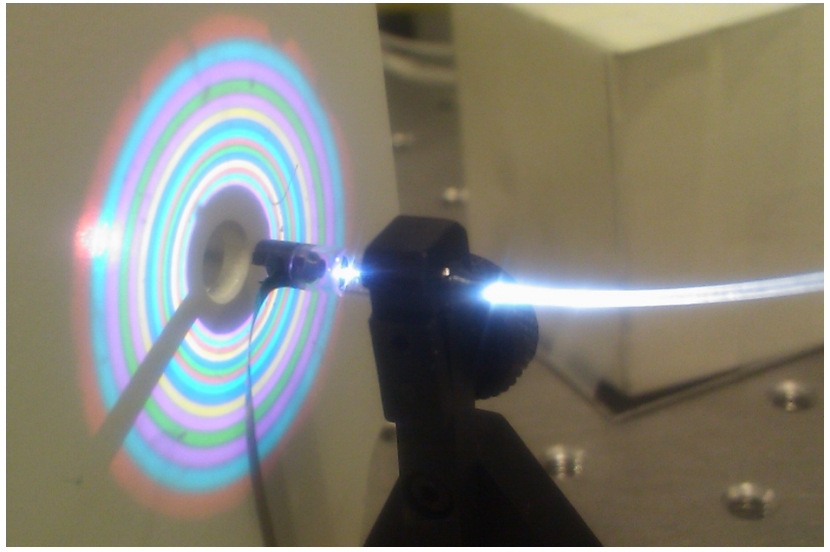
\includegraphics[height=.8\textheight ]{images/structuredLight}\\
		\scriptsize Structured light endoscope | Source: "An endoscopic 3D scanner based on structured light"
	\end{center}

\end{frame}



\begin{frame}{Structured Light Endoscopy}

	\begin{center}
		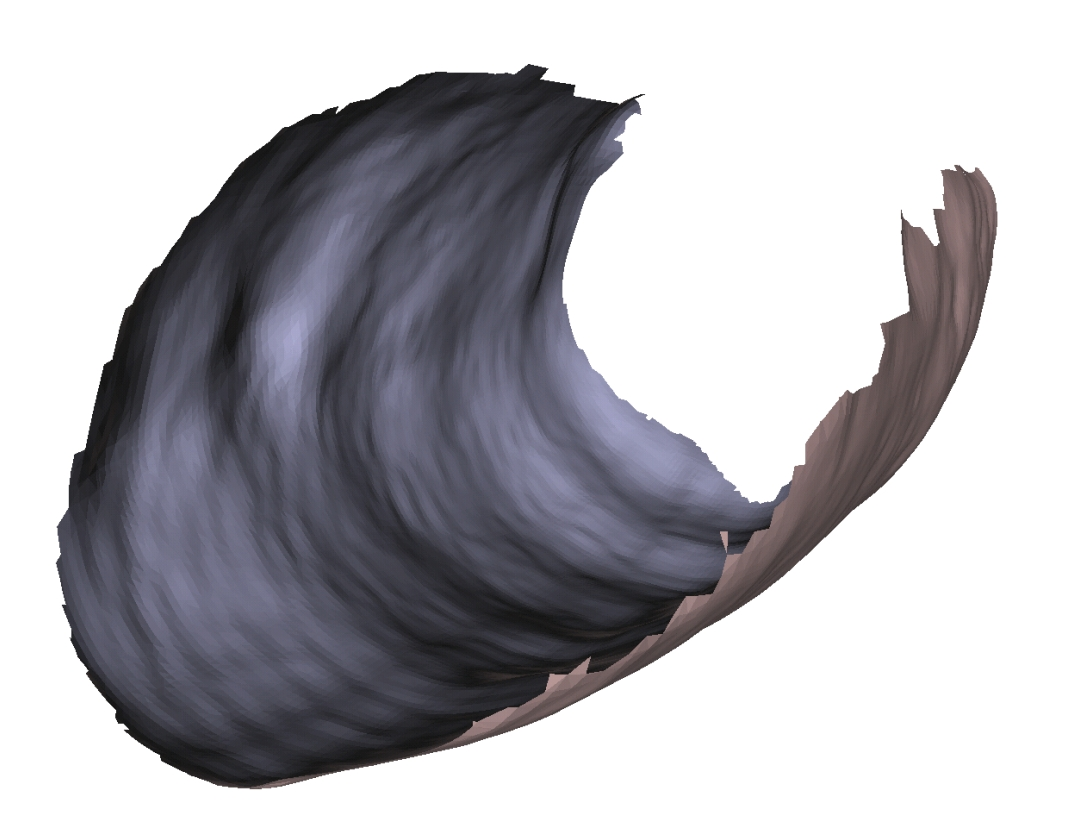
\includegraphics[height=.8\textheight ]{images/structuredLight1}\\
		\scriptsize Structured light data | Source: "An endoscopic 3D scanner based on structured light"
	\end{center}

\end{frame}



\begin{frame}{Structured Light Endoscopy}

	\textbf{Advantages:}
	\begin{itemize}
		\item[+] very accurate range data
		\item[+] almost independent of texture
	\end{itemize}
	\vspace{1em}
	\textbf{Disadvantages:}
	\begin{itemize}
		\item[-] low range image resolution
		\item[-] prototype only (no RGB data)
	\end{itemize}

\end{frame}



\begin{frame}[c]{Time-of-Flight Endoscopy}

	\begin{center}
		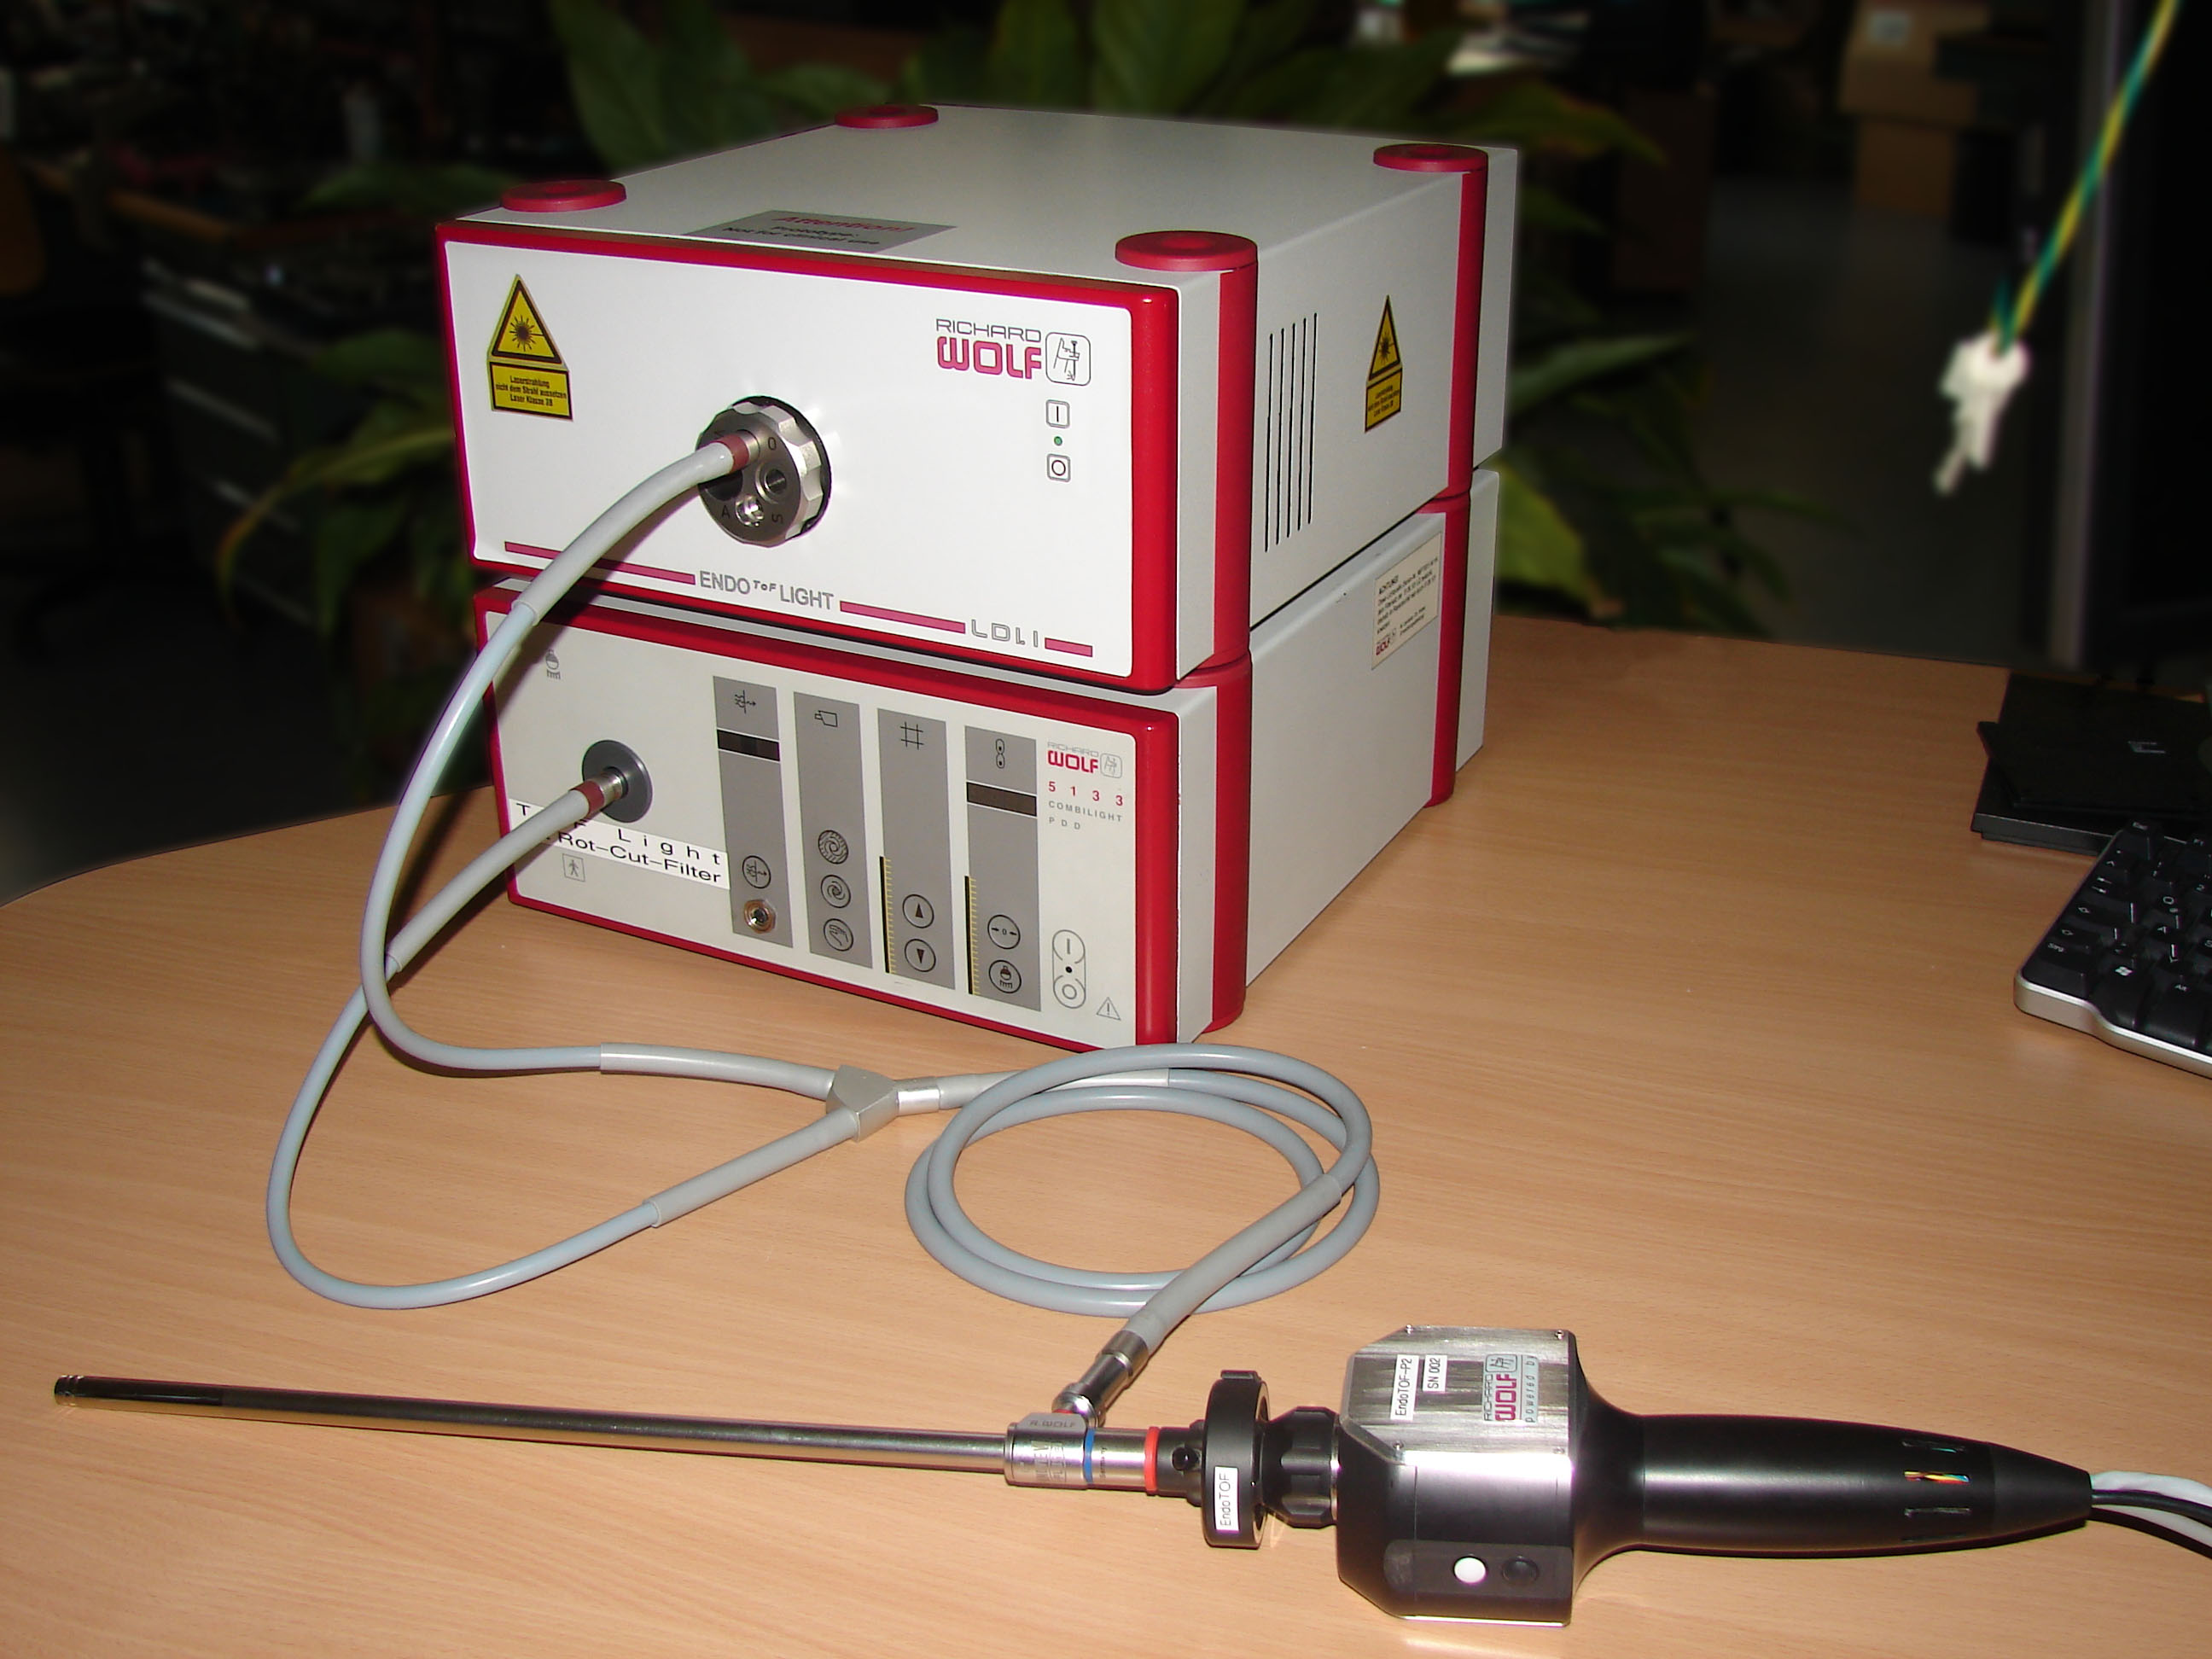
\includegraphics[height=.8\textheight ]{images/tof}\\
		\scriptsize Time-of-Flight/RGB endoscope | Source: Richard Wolf GmbH
	\end{center}

\end{frame}



\begin{frame}[c]{Time-of-Flight Endoscopy}

	\begin{center}
		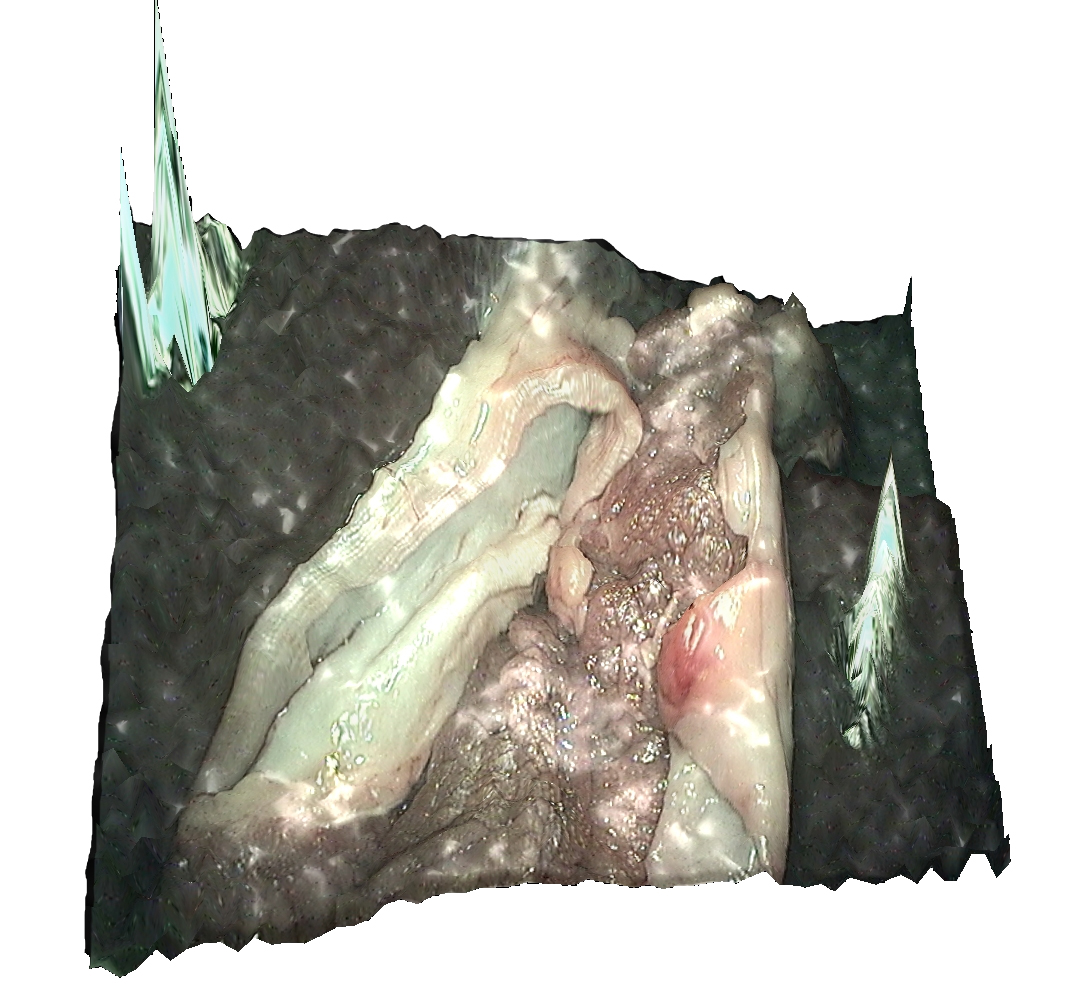
\includegraphics[height=.8\textheight ]{images/tof1}\\
		\scriptsize Hybrid ToF/RGB data | Source: LME, FAU
	\end{center}

\end{frame}



\begin{frame}{Time-of-Flight Endoscopy}

	\textbf{Advantages:}
	\begin{itemize}
		\item[+] constant range image resolution
		\item[+] independent of texture information
		\item[+] RGB and range information
	\end{itemize}
	\vspace{1em}
	\textbf{Disadvantages:}
	\begin{itemize}
		\item[-] low signal-to-noise-ratio
		\item[-] prototype only
	\end{itemize}

\end{frame}


\begin{frame}{Outline}
	\begin{itemize}
		\item History
		\item Setup
		\item Endoscopic Interventions
		\item NOTES
		\item 3-D Endoscopy
		      \bolditem Computer Assistance
		\item Future Trends
	\end{itemize}
\end{frame}



\begin{frame}{Computer Assistance (Definition)}

	\begin{myDefinition}
		\textit{Computer Assistance} in minimally invasive procedures allows improved visualization, data overlays or robot guidance to reduce the workload for the surgeon, improve safety or to reduce the operation time. Assistance means that so procedure is performed by computers only, the surgeon always has to keep the responsibility for the entire intervention.
	\end{myDefinition}
\end{frame}



\begin{frame}{da Vinci}

	\begin{center}
		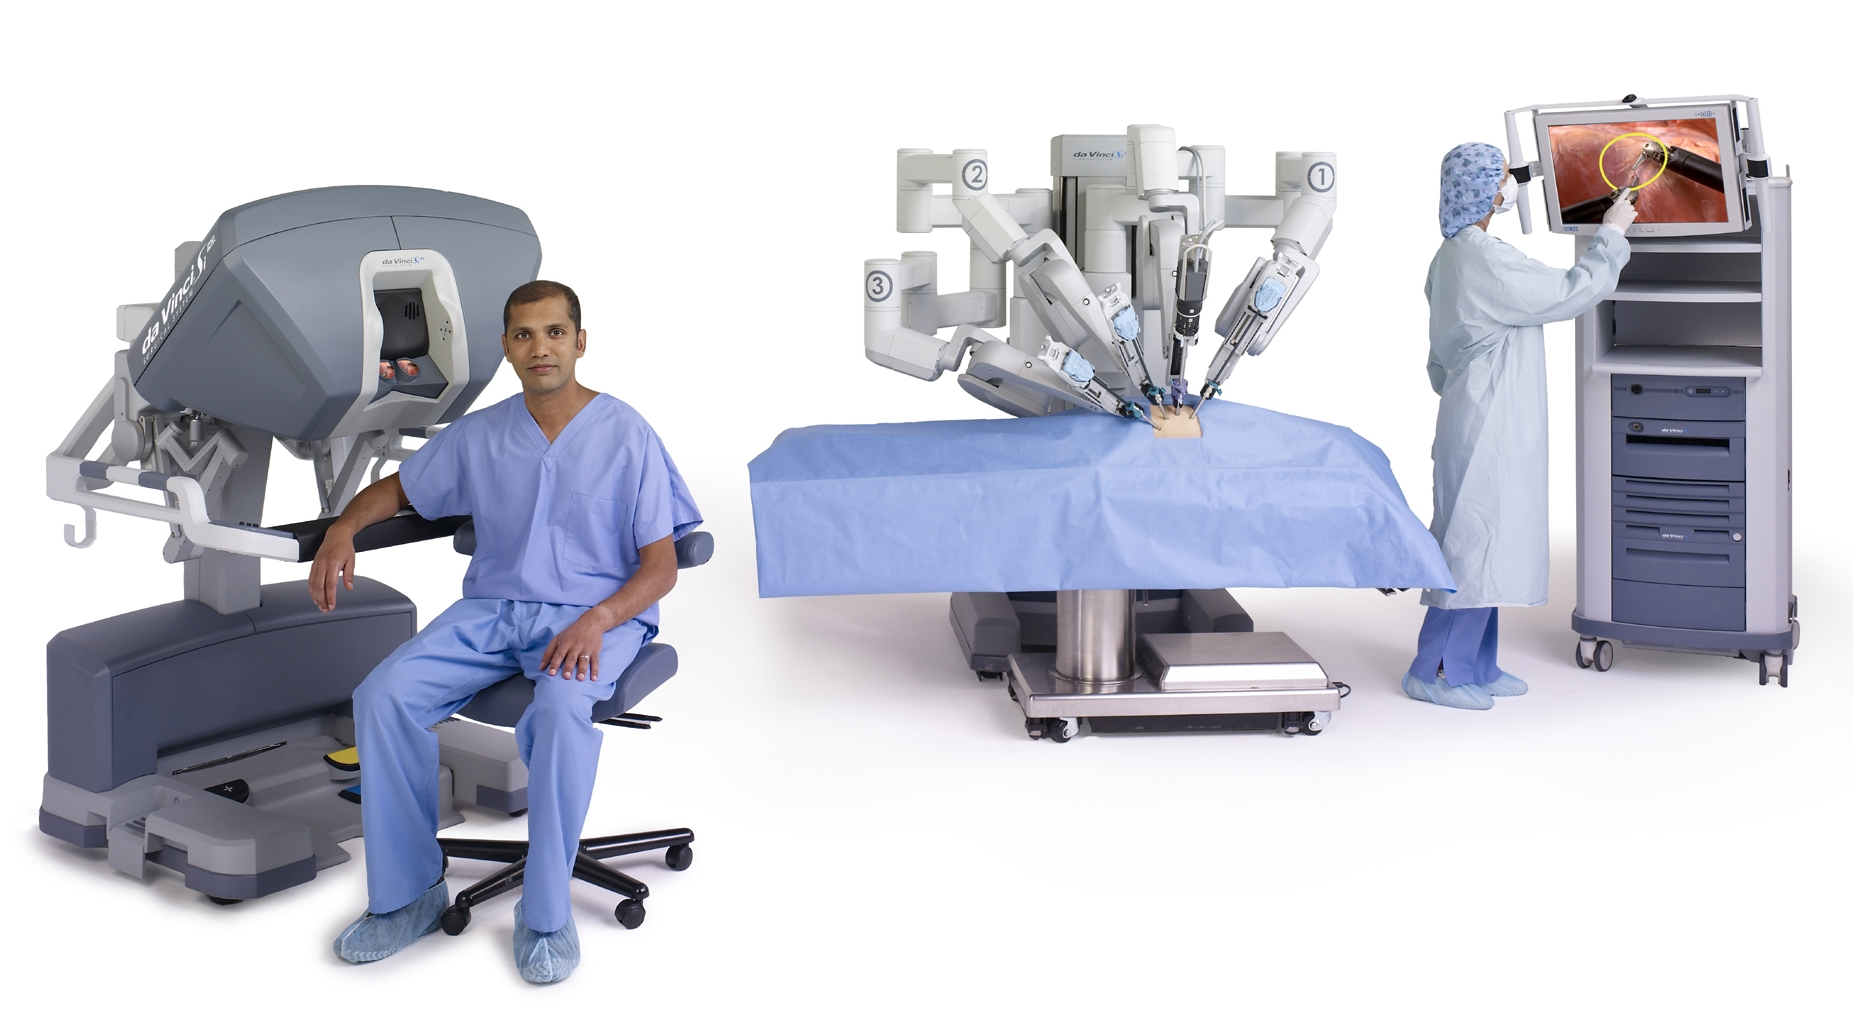
\includegraphics[height=.8\textheight ]{images/davinci}\\
		\scriptsize da Vinci setup | Source: Intuitive Surgical
	\end{center}

\end{frame}



\begin{frame}{da Vinci}

	\begin{itemize}
		\item \textit{Food and Drug Administration} (FDA) approved in 2000
		\item around 200.000 interventions in 2012
		\item around 2.000 units sold until January 2013
		\item acquisition costs of 2 million USD (+maintenance fees)
		\item only competitor ZEUS discontinued 2003
		\item provides 3-D stereo vision and intuitive controlling
		\item newest version adds a simulator with several virtual tutorials
		\item allows distant operations in theory (Dr. Marescaux has shown this in 2001, but keep in mind: latency is a big issue)
	\end{itemize}

\end{frame}



\begin{frame}{da Vinci}

	\textbf{Criticism}
	\begin{itemize}
		\item very high costs for hospitals
		\item surgeons have to learn to control the system
		\item software is proprietary and can not be modified
		\item no studies have shown real benefits for the patients
		\item there is no real competitor (monopoly!)
	\end{itemize}

\end{frame}



\begin{frame}{da Vinci Navigation}
	\begin{columns}[T]
		\begin{column}{0.55\textwidth}
			\vspace{2em}
			\centering
			\begin{itemize}
				\item both hands navigate different tools
				\item foot pedal allows to switch to camera control
				\item second surgeon can be connected with another terminal
				\item tools have all degrees of freedom like human hands
				      %		\item tools can be repositioned in null space
			\end{itemize}
		\end{column}
		\begin{column}{0.45\textwidth}
			\centering
			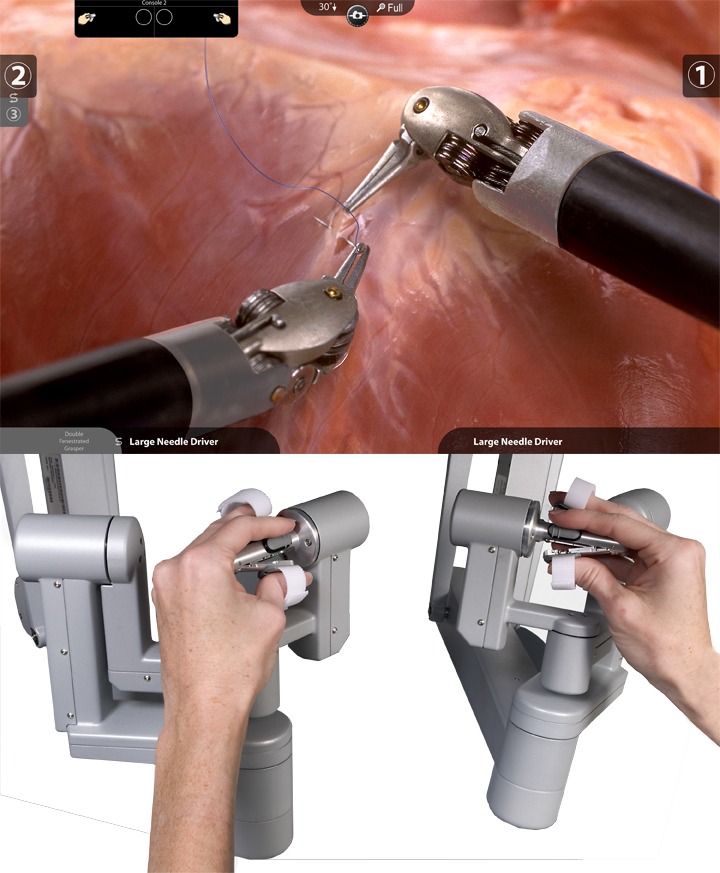
\includegraphics[height=.75\textheight ]{images/davinci1}\\
			\scriptsize da Vinci navigation | Source: Intuitive Surgical
		\end{column}
	\end{columns}


\end{frame}



\begin{frame}{Outline}
	\begin{itemize}
		\item History
		\item Setup
		\item Endoscopic Interventions
		\item NOTES
		\item 3-D Endoscopy
		\item Computer Assistance
		      \bolditem{} Future Trends
	\end{itemize}
\end{frame}



\begin{frame}{Future Trends}
	\begin{itemize}
		\item Fully automated procedures are still far away (legal issues, see autonomous driving)
		\item Realtime 3-D reconstruction will be used to provide augmented reality
		\item Ultra-thin endoscopes
		\item More NOTES and less scars?
		\item Data fusion becomes more and more important
		\item Higher image resolutions and improved data quality [show TOF/RGB
				      superresolution video here]

	\end{itemize}
\end{frame}


%
%\begin{frame}
%\frametitle{Future Trends}
%
%\begin{center}
%\includegraphics[height=.8\textheight ]{images/elysium}\\
%\scriptsize Medical pod | Source: Elysium
%\end{center}
%
%\end{frame}

\section{Questions?}

\section{Further Readings}%
\label{sec:further_readings}


\begin{frame}[t]{Further Readings}
	\begin{itemize}
		\item \fullcite{haase18}
	\end{itemize}
\end{frame}

\end{document}
